\documentclass[12pt]{article}
%\usepackage[utf8]{inputenc}
\usepackage{svg}
\usepackage{amsmath}
\usepackage{hyperref}
\usepackage{listings}
\usepackage{xcolor}
\usepackage{booktabs} % For prettier tables
\usepackage{multicol}
\usepackage{multirow}
\usepackage[shortlabels]{enumitem}
\usepackage{hyperref}
\usepackage{cleveref}
\usepackage{subcaption}
\usepackage{fancyhdr}
\usepackage{float}

\usepackage{longtable}
\usepackage{geometry}
%\geometry{margin=1in} % Adjust the page margins if needed

\usepackage{array}
\usepackage{ragged2e}
\usepackage{multirow}
\newcolumntype{P}[1]{>{\centering\arraybackslash}p{#1}} % center the column and justify its contents to the top in multirow tables
\newcolumntype{R}[1]{>{\RaggedLeft\arraybackslash}p{#1}} % Align column to the right in multirow tables

\definecolor{codegreen}{rgb}{0,0.6,0}
\definecolor{codegray}{rgb}{0.5,0.5,0.5}
\definecolor{codepurple}{rgb}{0.58,0,0.82}
\definecolor{backcolour}{rgb}{0.95,0.95,0.92}

\lstdefinestyle{mystyle}{
    backgroundcolor=\color{backcolour},   
    commentstyle=\color{codegreen},
    keywordstyle=\color{magenta},
    numberstyle=\tiny\color{codegray},
    stringstyle=\color{codepurple},
    basicstyle=\ttfamily\footnotesize,
    breakatwhitespace=false,         
    breaklines=true,                 
    captionpos=b,                    
    keepspaces=true,                 
    numbers=left,                    
    numbersep=5pt,                  
    showspaces=false,                
    showstringspaces=false,
    showtabs=false,                  
    tabsize=2
}

\lstset{style=mystyle}

% --- set footer and header ---
\renewcommand{\headrulewidth}{0pt}
%\renewcommand{\footrulewidth}{1pt}
\pagestyle{fancy}
\fancyhf{}

\setlength\headheight{16pt}
\setlength{\footskip}{50pt}
\lhead{\Title} %rightH title
\cfoot{\thepage}
% --- end footer and header ---

%----------EDIT COVER INFO HERE -----------------%

\def \DEPARTEMENT {Department of Media}
\def \COURSENUM {Data Science}
\def \COURSENAME {Master Thesis}
\def \REPORTTITLE {Reading and Understanding Annual Reports Using Large Language Models and Retrieval-Augmented Generation}

%------------------------------------------------%

\begin{document}

\pagenumbering{Roman}

\begin{titlepage}
    \vfill
    \begin{center}
        \hfill \\
        \Large{\DEPARTEMENT} \\
        \Large{\COURSENUM\;-\;\COURSENAME} \\
        \vfill
        \vfill
        \vfill
        \textbf{\LARGE{\REPORTTITLE}}
    \end{center}
    \vfill
    \vfill
    \vfill
    \vfill
    \vfill
    \begin{flushleft}
    \end{flushleft}
    \vfill
\end{titlepage}

%-----------------------------------------------%

%\tableofcontents
%\clearpage


\chapter{NBl. HS MSGWG Schl.-H. Nr. 6/2016 vom 20. Dezember 2016, S. 102 Tag der Bekanntmachung auf der Internetseite der Fachhochschule Kiel: 20. Oktober 2016 37 Anlage D (zu § 28 PVO)}
\\
\\
\\
\\
Erklärung \\

Ich versichere, dass ich die Masterarbeit "Reading and Understanding Annual Reports Using Large Language Models and Retrieval-Augmented Generation" selbständig und ohne unzulässige fremde Hilfe angefertigt habe und dass ich alle von anderen Autoren wörtlich übernommenen Stellen wie auch die sich an die Gedankengänge anderer Autoren eng anlehnenden Ausführungen meiner Arbeit besonders gekennzeichnet und die entsprechenden Quellen angegeben habe. Diese Arbeit hat noch keiner Prüfungsbehörde vorgelegen. \\
\\
Ort, Datum, Unterschrift
\\
\\
\\
\\
\\
Declaration\\


I certify that I have completed the Master's thesis “Reading and Understanding Annual Reports Using Large Language Models and Retrieval-Augmented Generation” independently and without unauthorized outside help and that I have specifically marked all passages taken verbatim from other authors as well as those closely based on the ideas of other authors in my work and have cited the corresponding sources. This thesis has not yet been submitted to any examination authority.\\
\\
Place, date, signature
\\
\\
\\
Kiel,    \DATE
%\end{flushright}

\newpage

\tableofcontents

\newpage

\pagenumbering{arabic}
\fancyfoot[C]{\thepage}

%%%%%%% Note %%%%%%%
% The placeholder text is heavily influenced by the ACM proceedings template.
%%%%%%%%%%%%%%%%%%%%

\section{Introduction}
Natural Language Processing (NLP) technologies have significantly transformed various industries, with the finance sector being one of the primary beneficiaries. These technologies streamline complex tasks, automate customer services, and enhance decision-making processes, making them indispensable in the modern financial landscape. At the forefront of this transformation are Large Language Models (LLMs) such as GPT-4 \cite{OpenAI.15Mar2023}, which represent a cutting-edge advancement in artificial intelligence, offering extensive capabilities to analyze and interpret vast amounts of unstructured financial data quickly and effectively.

Corporate reports, especially those like the SEC Form 10-K \cite{SECOfficeofInvestorEducationandAdvocacy.2021} filings, are critical documents for financial decision-making. They provide comprehensive information about a company's financial health and operational dynamics. However, these reports are often lengthy and complex, posing significant challenges for document processing and information extraction. This thesis aims to develop a method leveraging LLMs and Retrieval-Augmented Generation (RAG) to facilitate the easy reading and understanding of these financial reports.

Despite their potential, the practical application of LLMs in finance faces substantial challenges. One of the primary concerns is their tendency for hallucination \cite{Huang.9Nov2023}, where the model might generate plausible but factually incorrect information. This is particularly problematic in finance, where accuracy and reliability are paramount. Additionally, the high cost of continuously updating these models to keep pace with the rapidly changing financial landscape poses another significant obstacle.

Moreover, enhancing LLMs with factual knowledge remains an ongoing challenge. The demand for precise and up-to-date information is critical in finance, and the static nature of trained models often clashes with the dynamic financial environment. To address these issues, the development of hybrid models that combine the generative power of LLMs with real-time, verified data sources could be a potential solution. This integration would leverage the strengths of LLMs in understanding and processing language while ensuring the accuracy and reliability required in financial applications.

This thesis focuses on developing a Retrieval-Augmented Generation (RAG) system to facilitate the understanding of financial annual reports. By integrating LLMs with retrieval of recent information, the proposed system aims to provide accurate and contextually relevant responses to user queries \cite{Gao.18Dec2023}. The thesis emphasizes using open-source libraries, frameworks, and language models to develop a RAG system that can run locally on a user's work computer. This approach democratizes and popularizes the use of modern LLMs achievements.

The primary research questions guiding this thesis are:
\begin{enumerate}
\item How can open-source utilities (libraries and models) be effectively combined with information retrieval to enhance the question-answering and understanding of financial reports?
\item What are the results of the RAG pipeline with using open-source utilities on real-life finance domain specific questions?
\end{enumerate}

To address these questions, the study adopts the following methodology:
\begin{enumerate}
\item A comprehensive review of existing research and theoretical foundation on embeddings, LLMs, vectore storage, RAG systems, and their applications. 
\item Using open-source LLMs and frameworks to develop a RAG system that can process and analyze financial reports. The system will be designed to run locally (without using any API calls), ensuring cost-effectiveness.
\item Conducting experiments to assess the quality of the system's responses to real  financial queries. This includes testing the system on questions of varying complexity and specificity, as well as manual evaluation of its accuracy.
\end{enumerate}

Using LLM solutions in finance can be done through two main options: utilizing an API from LLM service providers or employing open-source LLMs. Companies like OpenAI, Google, and Microsoft offer LLM services through APIs, providing base language model capabilities with additional features tailored for specific use cases. For example, OpenAI’s APIs\footnote{\url{https://openai.com/index/openai-api/}} include functionalities for chat, SQL generation, code completion, and code interpretation. While there is no dedicated LLM service exclusively designed for finance applications, leveraging these general-purpose LLM services can be a viable option for common tasks.

Unlike using APIs, hosting and running open-source models require self-hosting. Similar to using LLM APIs, zero-shot or few-shot learning approaches can be employed with open-source models. Utilizing open-source models offers greater flexibility, as the model’s weights are accessible, and the model’s output can be customized for downstream tasks. Additionally, it provides better privacy protection as the model and data remain under the user’s control. However, working with open-source models also has its drawbacks. Reported evaluation metrics suggest a performance gap between open-source models and proprietary models \cite{Zhao.31Mar2023}. For certain downstream tasks, open-sourced models may not yield optimal performance.

One of the critical challenges in enhancing LLMs with factual knowledge is the need for precise and up-to-date information. Financial markets move rapidly, and developers need to leverage RAG to equip LLMs with current knowledge. Moreover, SEC filings are hard to index by search engines due to their data formats. Indexing is the process by which search engines (like Google or Microsoft Bing) collect, parse, and store data to make it quickly retrievable in response to a search query. For a document to be easily indexed, its content needs to be in a format that the search engine can easily read and understand. SEC filings are often submitted in complex and varied formats \cite{Zhang.18Feb2023}. Historically, these have included plain text, HTML, and even image formats. More recently, filings might use XBRL (eXtensible Business Reporting Language), a specialized format for business information. While XBRL is very useful for financial analysis, it can be complicated for search engines to parse correctly.

Moreover, financial documents are complex themselves and require careful processing and chunking of data. Developers need to experiment with different ways of transforming tables, determining relevant entities, and linking them to parent sections \cite{Zhang.18Feb2023}. There's a low tolerance for false positives in retrieving these documents since these numbers directly influence important decisions.

The infrastructure for RAG is evolving rapidly, with developers inundated with choices. There are over 15 vector stores\footnote{\url{https://db-engines.com/en/ranking/vector+dbms}} to choose from, some relational database management systems also provide vector storage capabilities, and an ever-changing list of embedding models on the MTEB Leaderboard\footnote{\url{https://huggingface.co/spaces/mteb/leaderboard}}. New ways to embed and retrieve information emerge constantly.

Using a locally running open-source LLM instead of relying on an API for retrieval tasks to extract information from text offers several advantages:
\begin{enumerate}
\item Relying on an API for large-scale text processing can result in substantial costs, especially as usage increases. Running an open-source LLM locally eliminates the need to pay for API calls, making it a cost-effective solution for companies with high-volume text processing needs.
\item Users can scale their local infrastructure based on their specific requirements without being constrained by API usage limits or facing unexpected costs associated with increased usage. This flexibility allows for better cost management and resource optimization.
\item Open-source LLMs often allow for fine-tuning on custom datasets, enabling companies to tailor the model to their specific domain or industry. This customization can lead to improved performance on tasks relevant to the unique requirements.
\end{enumerate}

The application of LLMs in finance holds immense promise, addressing tasks like fraud detection, financial sentiment analysis, price prediction and reasoning \cite{Li.28Sep2023}. LLMs come with a significant financial burden, being notably expensive to develop, train, and maintain. This cost factor raises practical challenges and limits accessibility for broader usage in various financial applications. Training costs for LLMs are a significant consideration. As of July, 2024, based on the number of GPU hours consumed and prices for AWS GPU usage, the estimated training costs of LLMs approximately are: FinGPT (finance domain specific model, fine-tuned on finance data): \$0.002 million, BloombergGPT: \$2.67 million, LLaMA2-7B: \$4.23 million\footnote{\url{https://github.com/AI4Finance-Foundation/FinGPT}}. 

Unlike traditional models, the RAG system offers a distinct edge by eliminating the need for frequent model retraining when new SEC filings become available. This characteristic saves valuable time and alleviates the resource-intensive process of retraining large language models, ensuring that the system remains up-to-date and adaptive without incurring the associated costs.

The proposed RAG system for interpreting and comprehending financial annual reports is tailored to serve the diverse needs of users within the finance sector. These users may include:
\begin{enumerate}
\item Private investors looking to analyze a company's financial reports before making investment decisions or tracking the performance of companies they already have stakes in.
\item Professional financial experts who can leverage the system to automate the extraction of relevant information, thereby saving time and enabling them to focus on companies that previously fell outside their scope due to time constraints.
\item SEC employees, who by law must review each company's report once every three years. The system will allow employees to save time, increase the frequency of report checks and improve quality
\end{enumerate}

This thesis refrains from creating a model for predictions, such as fraud detection and price predictions, which are already popular tasks. Instead, it focuses on the hypothesis that predictions should still be made by individuals.

\newpage
\section{Literature Review}
Retrieval-Augmented Generation (RAG) is a technique designed to enhance the performance of Large-Language Models (LLMs) by integrating external knowledge. This method has been extensively researched, exploring various configurations and applications. Key studies include a detailed analysis of RAG configurations \cite{Gao.18Dec2023}, highlighting their role in improving Natural Language Processing (NLP) tasks by reducing errors and enhancing factual accuracy. Several methods for context retrieval have been proposed to dynamically fetch documents, thereby improving the coherence of generated outputs \cite{Anantha.10Dec2023}. Other research has introduced advancements in RAG, such as reasoning chain storage and optimization strategies for retrieval, which broaden the scope and efficiency of RAG applications in LLMs \cite{Lewis.22May2020}. More recent work has compared RAG with LLM fine-tuning, finding that using both methods together improves their individual performances \cite{Balaguer.16Jan2024}.

Pre-trained LLMs store factual knowledge and achieve state-of-the-art results on NLP tasks but struggle with knowledge-intensive tasks and providing decision provenance. Combining parametric and non-parametric memory with generation improves knowledge-intensive task performance\cite{Lewis.22May2020}. The EDGAR-CORPUS dataset and edgar-crawler provide a financial NLP corpus excluding tables \cite{Loukas.2021}. Instruction Tuning explores task-specific tuning of LLMs in finance, highlighting diverse capabilities and future strategies for improvement \cite{Wang.31Dec2023}.

Recent frameworks like Self-Reflective Retrieval-Augmented Generation (SELF-RAG) enhance LLM quality and factuality through retrieval and self-reflection \cite{Asai.17Oct2023}. ITER-RETGEN synergizes retrieval and generation iteratively, improving relevance modeling for question answering tasks \cite{Shao.24May2023}.

In the financial domain, NLP applications include sentiment analysis, question answering, and stock market prediction. Advances in general-domain LLMs have motivated interest in Financial LLMs (FinLLMs), employing methods like mixed-domain LLMs with prompt engineering and instruction fine-tuned LLMs \cite{Lee.4Feb2024}.

Exploring the structure of financial reports is essential for establishing optimal principles for chunking. The complexity of document structures and content has led most research on financial reports to focus on identifying structural elements \cite{Yepes.5Feb2024}. Recent work includes DocLayNet \cite{Pfitzmann.2022}, which addresses document structures in U.S. SEC reports, and FinTabNet \cite{Zheng.}, which specifically focuses on table structures within these reports.

Most previous work has focused on understanding the layout of financial documents or specific snippets of reports. Recent research includes FinanceBench \cite{Islam.20Nov2023}, which proposes questions about financial report content and evidence snippets.

Corporate annual reports, especially SEC Form 10-K filings, are crucial for financial decision-making but are challenging due to their length and complexity. Machine Learning and Deep Learning techniques are being used to process these reports, improving accessibility for individual investors.

Financial domain-specific LMs are often built using general-domain LMs. Notable financial pre-trained LMs include FinBERT19 \cite{Araci.27Aug2019}, FinBERT-20 \cite{Shah.31Oct2022}, and FinBERT-21 \cite{ZhuangLiuDegenHuangKaiyuHuangZhuangLiJunZhao.2020}, all based on the BERT architecture. FinBERT-19, the first FinBERT model, was released for financial sentiment analysis and involved continual pre-training on a financial domain corpus after initial training on a general-domain BERT model. FinBERT-20 is a finance-specific BERT model pre-trained on a larger financial communication corpus. FinBERT-21, also BERT-based, was trained on both general and financial domain corpora and experimented with tasks such as Sentiment Analysis, Sentence Boundary Detection, and Question Answering \cite{Lee.4Feb2024}.

FLANG \cite{Shah.31Oct2022} is a domain-specific model trained using financial keywords and phrases for masking, following the training strategy of ELECTRA \cite{Clark.23Mar2020}. It introduces Financial Language Understanding Evaluation (FLUE), a collection of five financial NLP benchmark tasks: Sentiment Analysis, Headline Text Classification, Named Entity Recognition, Structure Boundary Detection, and Question Answering.

FinMA or PIXIU \cite{Xie.8Jun2023} consists of two fine-tuned LLaMA models with 7B and 30B parameters \cite{Touvron.27Feb2023}, using financial instruction datasets for various financial tasks. It is based on the Financial Instruction Tuning (FIT) dataset and includes tasks beyond FLUE, such as Stock Movement Prediction.

InvestLM \cite{Yang.15Sep2023} is a fine-tuned LLaMA model with 65B parameters, trained using a curated financial domain instruction dataset that includes Chartered Financial Analyst (CFA) exam questions, SEC filings, and financial NLP tasks. It extends beyond tasks covered by FinMA to include financial text summarization.

FinGPT \cite{Yang.9Jun2023} is an open-source, data-centric framework providing APIs for financial data sources, instruction datasets for financial tasks, and fine-tuned financial LLMs. It utilizes the Low-Rank Adaptation (LoRA) method for instruction fine-tuning.

BloombergGPT \cite{Wu.30Mar2023} is a closed-source FinLLM based on the BLOOM model \cite{Workshop.9Nov2022}, trained on both general and financial corpora, with financial data sourced from Bloomberg’s proprietary database. It covers both financial and general-purpose NLP tasks.

Recent advances in LLMs have opened new possibilities in finance. The paper 'Large Language Models in Finance: A Survey' \cite{Li.28Sep2023} reviews current approaches, including zero-shot and few-shot learning, domain-specific fine-tuning, and custom LLM training. It provides a decision framework for financial professionals to select appropriate LLM solutions based on their use case constraints.

Question Answering (QA) in finance involves retrieving or generating answers to questions from unstructured documents, requiring numerical reasoning across multiple formats. FiQA-QA \cite{Yang.23Aug2018} is an early Financial QA dataset for opinion-based QA. FinQA \cite{Chen.1Sep2021} and ConvFinQA \cite{Chen.8Oct2022} datasets involve hybrid QA, combining tabular and textual content for financial reasoning tasks.

Using 10-K forms, \cite{Ge.26Jan2023} measures regulatory barriers globally by fine-tuning BERT. \cite{Pasch.4Feb2022} fine-tuned BERT on various company-related text data for stock price prediction, resulting in StonkBERT, a transformer-based stock performance classifier. Analysts also use BERT for causal information classification or GPT-3.5 for creating quantitative datasets. Summarization and RAG improve accessibility for individual investors.

Major challenges in finance include utilizing internal data without privacy breaches and enhancing trust in FinLLMs' responses. Techniques like RAG \cite{Lewis.22May2020} help by providing LLMs with access to external knowledge, improving factual accuracy and reducing hallucination issues. RAG allows the use of internal data without retraining the entire model, ensuring privacy.

\newpage
\section{Theoretical Foundation}

\subsection{Embeddings}
Word embeddings are a class of techniques in NLP where words or phrases from a vocabulary are mapped to vectors of real numbers. The core idea behind word embeddings is to capture the semantic meaning of words such that words with similar meanings have similar representations. This transformation allows machine learning algorithms to leverage the geometric properties of the embeddings, making it easier to analyze and process textual data. In the field of information retrieval, the first-stage retrieval often relies on text embeddings to efficiently recall a small set of candidate documents from a large-scale corpus using approximate nearest neighbor search techniques. Embedding-based retrieval is also a crucial component of RAG \cite{Wang.31Dec2023}.

The concept of representing words as vectors isn't entirely new. Its roots can be traced back to the 1950s and 1960s, with foundational work by linguists and cognitive scientists. The theoretical underpinning of word embeddings is the distributional hypothesis, which posits that words occurring in similar contexts tend to have similar meanings. This idea, often summarized as "You shall know a word by the company it keeps" \cite{J.R.Firth.1957}, forms the basis for various embedding techniques. By analyzing the contexts in which words appear, it is possible to infer their semantic properties.

The early attempts to quantify semantic similarity between words led to the development of thesauri and semantic networks, such as WordNet, which organized words based on their meanings and relationships. However, these approaches were largely symbolic and didn't capture the continuous nature of semantic relationships \cite{GeorgeA.Miller.1995}.

In the 1980s and 1990s, the introduction of Latent Semantic Analysis (LSA) marked a significant shift. At its core, LSA relies heavily on Singular Value Decomposition (SVD), a linear algebra technique that decomposes a matrix into three other matrices, allowing the extraction of latent semantic information. Specifically, LSA applies SVD to a term-document matrix, where each row corresponds to a term (word) and each column corresponds to a document. The entries of this matrix typically represent some measure of the frequency or importance of each term in each document. By performing SVD on this matrix, LSA identifies a set of orthogonal vectors (singular vectors) that capture the underlying patterns of co-occurrence between terms and documents. These vectors are ordered by the amount of variance they explain in the original data, enabling LSA to reduce the dimensionality of the term-document space while preserving the most significant patterns of word usage across documents. The output of LSA is a set of latent semantic vectors, where each term and document is represented as a vector in a lower-dimensional continuous space. This representation allows LSA to capture the semantic relationships between words and documents based on their distributional patterns across the corpus. One significant limitation of LSA is its scalability to large vocabularies. The term-document matrix grows with the number of unique terms in the corpus, resulting in a computational challenge when applying SVD. SVD is computationally expensive, especially for matrices with high dimensionality, making it impractical to scale LSA to very large datasets or vocabularies. LSA operates under the bag-of-words assumption, which means it disregards the order and context of words within documents. As a result, LSA may struggle to capture fine-grained contextual nuances and subtle differences in meaning that depend on word order or syntactic structure.

LSA pioneered the use of linear algebra techniques like SVD to uncover latent semantic structures in text data. Despite its success in capturing semantic relationships and reducing dimensionality, LSA has notable limitations. These include challenges with handling large vocabularies, capturing contextual nuances, potential information loss during dimensionality reduction, and lack of adaptability to changing linguistic contexts. These limitations paved the way for more advanced techniques like word embeddings (e.g., Word2Vec, GloVe) and contextualized embeddings (e.g., ELMo, BERT), which aim to address these shortcomings and provide richer representations of language in NLP tasks.

Another traditional approach for text-based learning is via the Term Frequency - Inverse Document Frequency (TF-IDF) method, which can represent the document as a long numeric vector of TF-IDF scores for each word. The TF-IDF is the product of two statistics, term frequency and inverse document frequency. There are various ways for determining the exact values of both statistics. However, TF-IDF does not attempt to directly extract the latent semantic information within the text.

The early 2000s saw further advancements with the introduction of neural network-based models. Some works on a neural probabilistic language model demonstrated that distributed representations of words could improve language modeling tasks \cite{YoshuaBengioRejeanDucharmePascalVincentChristianJauvin.2003}. This laid the groundwork for subsequent developments in word embeddings, leading to the creation of more sophisticated models like Word2Vec and GloVe.

Word2Vec is one of the most influential models for learning word embeddings. uses neural networks to generate word embeddings through two architectures: Continuous Bag of Words (CBOW) and Skip-gram \cite{Mikolov.16Jan2013}.

In the CBOW model, the objective is to predict a target word based on its surrounding context words. Formally, given a context window of size c, the probability of a target word \(w_{t}\) given the context words \\ \(w_{t-c}, \ldots, w_{t-1}, w_{t+1}, \ldots, w_{t+c}\) is modeled as:\\
\[P(w_t \mid w_{t-c}, \ldots, w_{t-1}, w_{t+1}, \ldots, w_{t+c})\] \\
The training involves maximizing the log probability of the target word given its context over the entire corpus.

The Skip-gram model, on the other hand, reverses this approach. It aims to predict the context words given a target word. For a given word \(w_{t}\), the model maximizes the probability of its surrounding words: \\
\[P(w_{t-c}, \ldots, w_{t-1}, w_{t+1}, \ldots, w_{t+c}) \mid w_t) \] \\
The Skip-gram model has been found to perform well, especially on smaller datasets and for capturing rare word representations. 

Both variants utilize negative sampling or hierarchical softmax to efficiently approximate the softmax function over a large vocabulary, making the training process computationally feasible.

GloVe (Global Vectors for Word Representation), combines the strengths of the count-based and prediction-based approaches. The core idea behind GloVe is to construct a global co-occurrence matrix from the corpus and then factorize this matrix to obtain word vectors \cite{Pennington.2014}.

The objective function in GloVe is designed to capture the ratio of word co-occurrence probabilities. Specifically, given a word \(w_i\) and a context word \(w_j\), the ratio of their co-occurrence probabilities with another word \(w_k\) should be similar to the ratio of their co-occurrence probabilities with each other. This relationship is captured by the following cost function: \\
\[
J = \sum_{i,j=1}^{V} f(X_{ij})(w_i^T w_j + b_i + b_j - \log X_{ij})^2
\]\\
Here, \(X_{ij}\) denotes the co-occurrence count of words \(w_i\) and \(w_j\), \(b_i\) and \(b_j\) are bias terms, and \(f(X_{ij})\) is a weighting function that limits the influence of frequent co-occurrences. By optimizing this objective function, GloVe learns embeddings that incorporate both local context (like Word2Vec) and global statistical information from the entire corpus.

FastText, developed by Facebook's AI Research (FAIR) lab, extends the Word2Vec model by representing words as bags of character n-grams \cite{Joulin.6Jul2016}. This approach allows FastText to capture subword information, making it particularly effective for morphologically rich languages and rare word representations. The model learns embeddings for character n-grams and represents words as the sum of these embeddings. The training process for FastText is similar to that of Word2Vec, but with the additional step of generating n-grams for each word. This modification enables FastText to generalize better to unseen words and handle out-of-vocabulary words more gracefully.

The above methods learn only a single, static representation for each word, and do not take into consideration the phenomenon of polysemy, where a word can change its meaning depending on the context. The state-of-the-art (SOTA) pre-trained language models built on top of the very effective Transformer-based attention model, which can learn contextual word embeddings. These embeddings are dynamic in terms of the surrounding block or context of the word, so that the same word can get different representations that are most effective in capturing the lexical and semantic information \cite{Xia.14Jun2022}. 

ELMo (Embeddings from Language Models) generates word embeddings based on the entire context of a sentence using bidirectional LSTM networks. ELMo is a deep contextualized word representation model designed to improve various NLP tasks by providing rich word embeddings. The key idea behind ELMo is to use representations from a bi-directional language model (biLM) that are learned from a large corpus. These representations are context-sensitive, meaning that they can capture different meanings of words depending on their usage in different sentences \cite{Peters.15Feb2018}.

BERT (Bidirectional Encoder Representations from Transformers) further improves contextual understanding by using the Transformer architecture \cite{Devlin.11Oct2018}. BERT alleviates the unidirectionality constraint (for example, a left-to-right architecture, where every token can only attend to previous tokens in the self-attention layers of the Transformer model) by using a “masked language model” (MLM) pre-training objective. The masked language model randomly masks some of the tokens from the input, and the objective is to predict the original vocabulary id of the masked word based only on its context. BERT’s model architecture is a multi-layer bidirectional Transformer \cite{Vaswani.12Jun2017} encoder with two model sizes: BERT(base)/  BERT(large) with 12/ 24 layers (transformer blocks), 768/ 1024 hidden size, 12/ 16 self-attention heads, 110M/ 340M total parameters, кespectively. 

BERT pre-trains a deep bidirectional model on large corpora, capturing intricate word relationships and achieving state-of-the-art performance on various NLP benchmarks. We will discuss the architecture of Transformers in more detail in the subsection of language models.

Recent research has introduced prominent embedding models such as AngIE, Voyage, BGE, etc, which are benefit from multi-task
instruct tuning. Hugging Face’s MTEB leaderboard evaluates embedding models across 8 tasks, covering 58 datasests. Additionally, C-MTEB focuses on Chinese capability, covering 6 tasks and 35 datasets. By the time of the experiments (March 2024), the small BGE model ('bge-small-en-v1.5') ranked high in the MTEB Leaderboard ranking \cite{Gao.18Dec2023}.

'bge-small-en-v1.5' uses BERT general architecture with 33.2 mln parameters, 512 context length (maximum tokens) and 384 embedding length (dimensions)\footnote{\url{https://ollama.com/znbang/bge:small-en-v1.5-f32/blobs/bf40c42ad7d8}}. The model uses a WordPiece tokenizer\footnote{\url{https://huggingface.co/BAAI/bge-small-en-v1.5/raw/main/tokenizer.json}}, which uses subword tokenization method, when single word might be broken down into smaller units called subtokens (similar to Byte Pair Encoding (BPE)).

BGE (BAAI General Embeddings) provides a family of welltrained models for English and Chinese general text embeddings. There are three optional model sizes: small (24M), base (102M), and large (326M). BGE model series have received more than 20 million downloads from HuggingFace since its release on August 2023, making it one of the most popular embedding models in the world. They have been integrated by the major RAG and text-embedding frameworks in the world, such as Langchain, LLamaIndex and Huggingface. The code-base also receives nearly 5,000 stars on GitHub \cite{Xiao.14Sep2023}.


\subsection{Transformers}
Recent advances in artificial intelligence, especially in natural language processing, have led to the development of powerful LLMs like ChatGPT. Over the past few decades, language model architectures have undergone significant evolution. Initially, n-gram models represented word sequences assuming that the probability of the next word depends solely on the preceding (n − 1) words. For example, in a bigram model, the probability of a word is only conditioned on the previous word. Later, Recurrent Neural Network (RNN)-based models like Long Short-Term Memory networks (LSTM) emerged as neural network solutions, which are capable of capturing long-term dependencies in sequential data \cite{.2023}.

A significant breakthrough came in 2017 with the introduction of the Transformer model \cite{Vaswani.12Jun2017}. Transformers are based on a processing concept called self-attention, an attention mechanism relating different positions of a single sequence in order to compute a representation of the sequence. Self-attention has been used successfully in a variety of tasks including reading comprehension, abstractive summarization, textual entailment and learning task-independent sentence representations. End-to-end memory networks are based on a recurrent attention mechanism instead of sequencealigned recurrence and have been shown to perform well on simple-language question answering and language modeling tasks. The Transformer is the first model relying entirely on self-attention to compute representations of its input and output without using sequence aligned RNNs or convolution \cite{AustinHuangSurajSubramanianJonathanSumKhalidAlmubarakandStellaBiderman..2022}.

The Transformer architecture is composed of an encoder-decoder structure, although many applications, such as BERT, use only the encoder, and others, like GPT, use only the decoder. The architecture is highly modular and consists of the following key components:
\begin{enumerate}
\item The Encoder processes the input sequence and generates a set of context-aware representations. It consists of multiple identical layers, each containing two main sub-layers Multi-Head Self-Attention Mechanism (allows the model to focus on different parts of the input sequence simultaneously by creating multiple attention heads. Each head computes a different attention distribution, and their outputs are concatenated and linearly transformed) and Position-Wise Feed-Forward Network(applies two linear transformations with an activation function in between to each position in the sequence independently, enhancing the model's ability to capture non-linear relationships. Each sub-layer is followed by layer normalization and residual connections to facilitate training and improve model stability.
\item The decoder generates the output sequence, often in an autoregressive manner, meaning it predicts the next word based on previously generated words and the encoder's context-aware representations. Similar to the encoder, the decoder consists of multiple identical layers, each containing three main sub-layers: Masked Multi-Head Self-Attention Mechanism (ensures that the prediction for a particular position depends only on the preceding positions, preserving the autoregressive property), Multi-Head Attention Mechanism (allows the decoder to attend to the encoder's output, integrating information from the input sequence) and Position-Wise Feed-Forward Network (operates similarly to its counterpart in the encoder). Like the encoder, each sub-layer in the decoder is followed by layer normalization and residual connections.
\item Since the Transformer does not inherently capture the order of words (due to its parallel processing nature), positional encoding is added to the input embeddings. This encoding provides information about the position of each word in the sequence, enabling the model to utilize the order of words. \cite{Vaswani.12Jun2017}
\end{enumerate}

The Transformer model employs a layered structure that includes multiple layers of self-attention mechanisms and fully connected neural networks in both its encoder and decoder components, as illustrated in the \autoref{fig:transformer}.

\begin{figure}[h!]
\centering
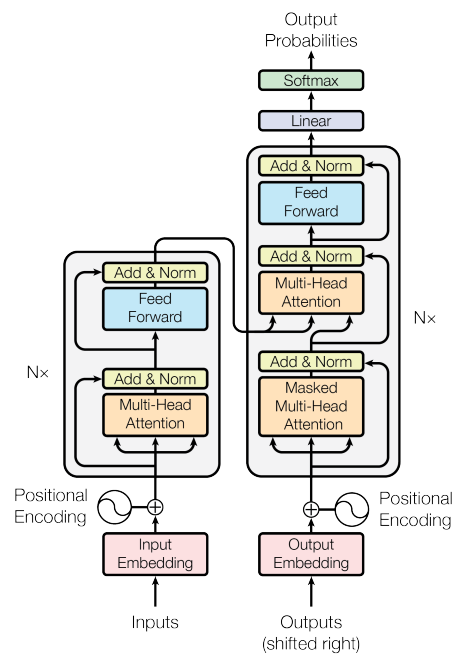
\includegraphics[width=0.5\textwidth]{Figures/transformer.png}
\caption{The Transformer architecture \cite{Vaswani.12Jun2017}.}
\label{fig:transformer}
\end{figure}

The original Transformer model architecture, as described in the paper \cite{Vaswani.12Jun2017}, comprises a stack of 6 identical layers for the encoder. Each encoder layer includes two sub-layers: the first is a multi-head self-attention mechanism, and the second is a position-wise fully connected feed-forward network. Every sub-layer in the encoder, along with the embedding layers, generates outputs with a dimensionality of 512.

Similarly, the decoder consists of a stack of 6 identical layers. Each layer in the decoder has the same two sub-layers as the encoder layers, with an additional third sub-layer. This third sub-layer performs multi-head attention over the output of the encoder stack. Multi-head attention is a module for attention mechanisms which runs through an attention mechanism several times in parallel. The independent attention outputs are then concatenated and linearly transformed into the expected dimension \cite{Vaswani.12Jun2017}.

Attention allows a network to give different weights to different inputs, with weighting coefficients that themselves depend on the input values, thereby capturing powerful inductive biases related to data. These models are known as transformers because they transform a set of vectors in some representation space into a corresponding set of vectors, having the same dimensionality, in some new space. The goal of the transformation is that the new space will have a richer internal representation that is better suited to solving downstream tasks. One major advantage of transformers is that transfer learning is very effective, so that a transformer model can be trained on a large body of data and then the trained model can be applied to many downstream tasks using some form of fine-tuning. Transformers can be trained in a self-supervised way using unlabelled data, and especially well suited to GPU allowing models having of the order of a trillion parameters to be trained in reasonable time. \cite{Bishop.2024}

The Generative Pre-trained Transformer (GPT) models, developed by OpenAI, are among the most prominent LLMs. GPT-2 demonstrated the power of unsupervised pre-training on diverse text corpora followed by fine-tuning on specific tasks. GPT-3, with 175 billion parameters, significantly advanced this approach, enabling highly coherent text generation and impressive zero-shot and few-shot learning capabilities \cite{Brown.28May2020}. In November 2022, OpenAI released the conversation model ChatGPT, based on the GPT models. And in March 2023 GPT-4 was
released, which extended the text input to multimodal signals (text, images, audios) \cite{Zhao.31Mar2023}.

The collection of LLaMA models were introduced by Meta AI in February, 2023, consisting of four sizes, ranging from 7B to 65B
parameters. \cite{Touvron.27Feb2023}. LLaMa results show that it is possible to achieve state-of-the-art performance by training
exclusively on publicly available data, without
resorting to proprietary datasets and moreover LLaMA-13B outperforms GPT-3 while being more than 10× smaller. In July, 2024 Meta introduced Llama 3.1 model with 128K tokens context length with three sizes 8B, 70B and a flagship model with 405B parameters. Llama 3.1 405B delivers comparable quality to leading language models such as GPT-4 on a plethora of tasks (general knowledge, steerability, math, tool use, and multilingual translation)\footnote{\url{https://ai.meta.com/research/publications/the-llama-3-herd-of-models/}}.  

The phi-3-mini model from Microsoft is a transformer decoder architecture, unlike the full Transformer architecture (which consists of both encoder and decoder components), the decoder-only architecture focuses on generating text by predicting the next word in a sequence based on the preceding context. The model's default context length is 4K tokens, which means the model can consider up to 4096 tokens of input context when making predictions \cite{Abdin.22Apr2024}. The phi-3-mini model is built using a block structure that is similar to the Llama-2 model \cite{Touvron.18Jul2023}. This ensures compatibility and ease of adaptation for tools and techniques developed for Llama-2. The model uses the same tokenizer with vocabulary size of 320641. The tokenizer is responsible for converting text into tokens that the model can process. The vocabulary size indicates the number of unique tokens the model can recognize and generate. This large vocabulary size helps the model handle a diverse range of words and phrases.

The model uses 3072 hidden dimension (refers to the size of the hidden layers in the model, indicates the number of units in each hidden layer, which affects the model's capacity to learn and represent complex patterns in the data), 32 heads (determines how many different attention distributions are computed. Using 32 heads means that the model can focus on 32 different aspects of the input context simultaneously, enhancing its ability to capture nuanced relationships between tokens) and 32 layers stacked on top of each other (each layer contains its own set of parameters and contributes to the model's depth, enabling it to learn hierarchical representations of the input data). 

The model is trained using bfloat16 (Brain Floating Point, a 16-bit floating-point format provides a good balance between computational efficiency and numerical precision) for a total of 3.3T tokens (a larger training corpus provides the model with more diverse language patterns and knowledge, improving its ability to generate high-quality text). Developers utilized high quality training data to improve the performance of small language model. Such method allowed to reach the level of highly capable models such as GPT-3.5 or Mixtral with only 3.8B total parameters (while Mixtral has 45B total parameters). Phi-3 model's training data consists of heavily filtered publicly available web data from various open internet sources, as
well as synthetic LLM-generated data. Thanks to its small size, phi3-mini can be quantized to 4-bits so that it only occupies ≈ 1.8GB of memory. \cite{Abdin.22Apr2024}

In terms of LLM capabilities, while phi-3-mini model achieves similar level of language understanding and reasoning ability as much larger models, it is still fundamentally limited by its size for certain tasks. The model simply does not have the capacity to store too much “factual knowledge”. Moreover, developers have identified certain limitations, particularly with questions necessitating high-level reasoning abilities. Additionally, the model has been observed to occasionally generate ungrounded outputs, making it potentially unreliable in sensitive areas, such as finance. Such weakness can be resolved by augmentation with a search engine. \cite{Abdin.22Apr2024}


\subsection{Vector Databases}
A vector database is a database designed to store data as high-dimensional vectors, which mathematically represent features or attributes. Each vector comprises numerous dimensions, ranging from tens to thousands, depending on the data's complexity and detail. These vectors are typically created by applying an embedding function to the raw text \cite{Han.18Oct2023}. 

Vector databases function by building an index for all vectors contained within the database. This index is organized according to the vectors' attributes and their similarities. When a query is made to retrieve a vector, the database searches the index to find the most similar vectors and returns them as results. This approach allows for quick and efficient vector retrieval, even in large and complex databases. 

There are two primary approaches for searching in vector databases: Nearest Neighbor Search (NNS) and its variant, Approximate Nearest Neighbor Search (ANNS).

NNS is an optimization problem focused on identifying the point in a given dataset that is closest or most similar to a specified query point. Closeness is typically evaluated using a dissimilarity function, where larger function values indicate less similarity. For example, NNS can be utilized to locate documents similar to a specified document based on topic and sentiment. NNS algorithms usually employ exact or deterministic methods. Some common techniques include: "k-d tree" method partitions the space into regions by splitting along one dimension at a time; "Ball tree" approach encloses groups of points within hyperspheres. These methods visit only the regions that may contain the nearest neighbor, based on certain distance bounds or criteria \cite{Han.18Oct2023}.

ANNS, in contrast, allows for some approximation or error in the search results, trading off accuracy for increased speed and space efficiency. This approach is particularly advantageous for handling large-scale and high-dimensional data. ANNS methods use more probabilistic or heuristic strategies, such as: "Locality-sensitive hashing (LSH)" maps similar points to the same or nearby buckets with high probability; "Best bin first" visits regions in order of their distance to the query point and stops after examining a fixed number of regions or points; "Hierarchical navigable small world (HNSW)" follows edges that lead to closer points in a graph with different levels of coarseness \cite{Han.18Oct2023}.

The primary difference between NNS and ANNS algorithms lies in their design principles. NNS algorithms organize the data into exact structures and traverse these structures to find the nearest neighbor deterministically. ANNS algorithms use approximate structures and probabilistic methods to quickly find a close, but not necessarily the exact, nearest neighbor.
Any data structure or algorithm that supports NNS can generally be adapted for ANNS, offering flexibility for various search requirements. This adaptability ensures that vector databases can efficiently handle diverse and complex queries, making them suitable for a wide range of applications in fields like image retrieval, document clustering, and recommendation systems \cite{Han.18Oct2023}.

Hierarchical Navigable Small World (HNSW) is an advanced method for approximate nearest neighbor search in high-dimensional vector collections. It employs a graph structure where nodes represent vectors and edges denote similarity or distance. The algorithm uses a greedy search strategy, starting from a random point and moving to its nearest neighbor until no closer point is found. HNSW follows the following formula for finding the nearest neighbor of a point p in the graph using a random walk:
\[
\arg\min_{q \in N(p)} d(p, q)
\]
where \(N_p\) is the set of neighbors of \(p\) in the graph, and
\(d\) is a distance function, such as Euclidean distance or cosine
distance.

Adding edges to the graph follows a heuristic where points closer to a node than its current neighbors are connected:
\[
\forall q \in \mathcal{N}(p), \forall r \in \mathcal{N}(q), \text{ if } d(p, r) < d(p, q), \text{ then add edge}(p, r)
\]
where \(N_p\) and \(N_q\) are the sets of neighbors of \(p\) and
\(q\) in the graph, respectively, and \(d\) is a distance function.

HNSW organizes vectors into layers with different densities and distances, controlled by a parameter \(M\). Higher layers contain fewer nodes with longer edges, while lower layers have more nodes with shorter edges. Search begins at the highest layer, progressively refining candidates at each layer until the nearest neighbor is found. The formula for assigning a point \(p\) to a layer \(l\) using a random probability is:
\[
\Pr[p \in l] = \begin{cases}
1 & \text{if } l = 0, \\
\frac{1}{M} & \text{if } l > 0.
\end{cases}
\]
where \(M\) is the parameter that controls the maximum number of neighbors for each point in each layer. The algorithm assigns \(p\) to layer \(l\) with probability \(\Pr[p \in l]\), and stops when it fails to assign p to any higher layer. The formula for searching for the nearest neighbor of a query point \(q\) in the hierarchical graph is:
\[
\min_{p \in C(q)} d(q, p)
\]
where \(C_q\) is the set of candidate points obtained by
traversing each layer of the graph from top to bottom and
retrieving all the points that are closer than the current best
distance.

Key advantages of HNSW include its ability to handle various distance metrics, adapt to dynamic datasets, and achieve high accuracy with low memory usage compared to tree-based or hash-based methods. However, its performance depends on factors like vector dimensionality, layer count, neighbor count, and query hop count, impacting trade-offs between accuracy and efficiency \cite{Han.18Oct2023}.

Several open-source vector databases are available under Apache 2.0 or MIT licenses, including Chroma, Faiss, Marqo, Vespa, Qdrant, LanceDB, and Milvus. Additionally, traditional databases such as OpenSearch, ClickHouse (a column-oriented DBMS), PostgreSQL, and Cassandra now offer support for vector search. Although we did not conduct an in-depth analysis of these databases, we selected ChromaDB due to its simplicity and ease of use.

ChromaDB's straightforward integration makes it a good choice for our purpose, allowing us to focus on our core research objectives without being encumbered by complex database configurations. ChromaDB utilizes SQLite to store vectors in its in-memory version. SQLite, a file-based relational database, inherently lacks support for vector data. When a document is added to a collection, ChromaDB employs an embedding function to generate vectors for the document. For each collection, an index is constructed using the HNSW (Hierarchical Navigable Small World) approximate nearest neighbor search algorithm. When a text string is queried within a collection, ChromaDB generates vectors for the string using the same embedding function. It then searches the index for the k nearest neighbors, with k specified in the query. The index maintains UUIDs for the documents, which are used to retrieve the corresponding text strings.


\subsection{Retriever-Augmented Generation}
LLMs have demonstrated impressive performance, yet they still encounter notable challenges, particularly with tasks that require specialized knowledge or up-to-date information. A common issue is that they may produce "hallucinations"—inaccurate or fabricated information—when faced with queries that extend beyond their training data or require current facts. To address these limitations, RAG has been developed to improve LLMs. RAG enhances the capabilities of LLMs by retrieving relevant sections from an external knowledge base based on semantic similarity. This approach helps mitigate the generation of factually incorrect content by incorporating accurate external information. The adoption of RAG in LLMs has become widespread, positioning it as a crucial technology for advancing chatbots and making LLMs more effective and reliable for real-world applications \cite{Gao.18Dec2023}. 

The field of RAG has evolved swiftly in recent years, exhibiting several distinct phases of development in the context of large models. Initially, RAG emerged alongside the rise of the Transformer architecture, focusing on improving language models by integrating additional knowledge through Pre-Training Models (PTM). This early phase was dedicated to advancing pre-training methods and laying a solid foundation. The introduction of ChatGPT marked a significant turning point, showcasing advanced in-context learning (ICL) capabilities. This development prompted a shift in RAG research toward enhancing the provision of relevant information for LLMs, enabling them to handle more complex and knowledge-intensive tasks during the inference phase. As a result, RAG research experienced rapid advancements. Over time, improvements in RAG extended beyond just the inference stage and began to integrate with techniques for fine-tuning LLMs, reflecting a broader evolution in the field \cite{Gao.18Dec2023}.

A typical application of RAG is illustrated in the \autoref{fig:RAG}:
\begin{figure}[h!]
\centering
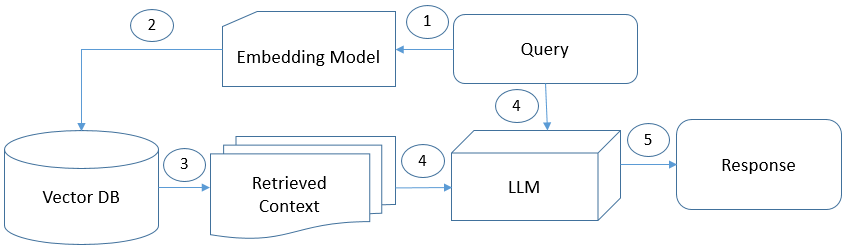
\includegraphics[width=1\textwidth]{Figures/RAG.png}
\caption{A typical RAG architecture}
\label{fig:RAG}
\end{figure}


Here, the user initiates the process by submitting a query (question or request). The query is then passed through an embedding model, which transforms the text data into a numerical representation. This allows the model to identify similar text passages within the document collection. The embedding model interacts with a vector database to retrieve relevant documents or passages. The vector database efficiently stores and retrieves information based on the numerical representations generated by the embedding model. The retrieved documents or passages that are most relevant to the query are then incorporated into the workflow. The retrieved context is presented, along with the original query, to a LLM. LLMs are trained on massive amounts of text data and are adept at understanding and responding to natural language. In the RAG workflow, the LLM leverages the retrieved context to generate a comprehensive and informative response to the user’s query. Finally, the LLM’s response is provided to the user.

Mathematically, the task of the RAG system can be formulated as follows.  Given input \(X\) and an accessible corpus containing a large amount of knowledge documents \(C = \{d_1, \ldots, d_N\}\), the system is expected to generate the output \(Y\). The entire framework is divided into a retriever \(R\)
and a generator \(G\). The retriever \(R\) aims to retrieve
the top-K documents \(D = \{d_{r1}, \ldots, d_{rk}\}\) that are
relevant to the input \(X\) from the corpus \(C\). Based on the input \(X\) and the retrieved results \(D\), the generator \(G\) is responsible for generating the output \(Y\). This framework can be formulated as:

\[P(Y|X) = P(D|X)P(Y, D|X)\]

It shows that the retriever and generator are seamlessly coupled, exhibiting low risk tolerance. Any unsuccessful retrieval can result in an unsatisfactory response, regardless of the impressive abilities of the generator \cite{Yan.29Jan2024}.

The RAG research paradigm is continuously evolving, and it may categorized into three stages: Naive RAG, Advanced RAG, and Modular RAG. Despite RAG method are cost-effective and surpass the performance of the native LLM, they also exhibit several limitations. The development of Advanced RAG and Modular RAG is a response to these specific shortcomings in Naive RAG. \cite{Gao.18Dec2023}

The Naive RAG research paradigm represents the earliest methodology, which gained prominence shortly after the widespread adoption of ChatGPT. The Naive RAG follows a traditional process that includes indexing, retrieval, and generation, which is also characterized as a “Retrieve-Read” framework. 

Indexing starts with the cleaning and extraction of raw data in diverse formats, which is then converted into a uniform plain text format. To accommodate the context limitations of language models, text is segmented into smaller, digestible chunks. Chunks are then encoded into vector representations using an embedding model and stored in vector database. This step is crucial for enabling efficient similarity searches in the subsequent retrieval phase. 

Upon receipt of a user query, the RAG system employs the same encoding model utilized during the indexing phase to transform the query into a vector representation. It then computes the similarity scores between the query vector and the vector of chunks within the indexed corpus. The system prioritizes and retrieves the top K chunks that demonstrate the greatest similarity to the query. These chunks are subsequently used as the expanded context in prompt. 

The posed query and selected documents are synthesized into a coherent prompt to which a large language model is tasked with formulating a response. The model’s approach to answering may vary depending on task-specific criteria, allowing it to either draw upon its inherent parametric knowledge or restrict its responses to the information contained within the provided documents \cite{Gao.18Dec2023}.

Naive RAG approaches face several significant challenges. During the retrieval phase, issues with precision and recall often arise, leading to the selection of irrelevant or mismatched chunks and missing important information. In the response generation phase, the model might produce hallucinations—content that is not supported by the retrieved context. This stage can also suffer from problems such as irrelevance, toxicity, or bias in the generated responses, which undermines the overall quality and reliability. Combining the retrieved information with the specific task at hand can be difficult, occasionally resulting in fragmented or incoherent responses. Additionally, there may be redundancy when similar information is retrieved from multiple sources, causing repetitive outputs. Assessing the significance and relevance of different passages, and maintaining stylistic and tonal consistency, further complicates the process. Moreover, a single retrieval based on the initial query might not provide sufficient context. There is also a risk that generation models may excessively rely on the retrieved information, producing outputs that merely restate the retrieved content without offering new insights or synthesis\cite{Gao.18Dec2023}.

Advanced RAG introduces specific improvements to overcome the limitations of Naive RAG. Focusing on enhancing retrieval quality, it employs pre-retrieval and post-retrieval strategies. The typical advanced RAG architecture is shown in \autoref{fig:advanced_arch}.\\ 
\begin{figure}[h!]
\centering
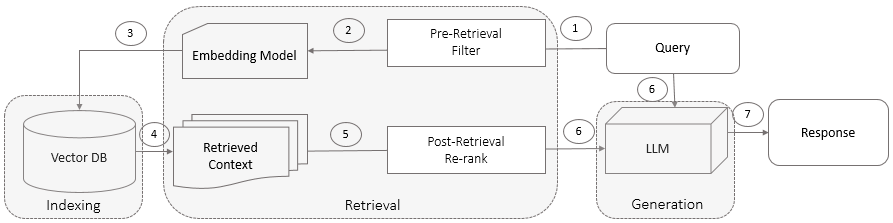
\includegraphics[width=1\textwidth]{Figures/advanced_arch.png}
\caption{An advanced RAG architecture}
\label{fig:advanced_arch}
\end{figure}

In the pre-retrieval stage, the main objectives are to optimize both the indexing structure and the original query. Improving the indexing involves enhancing the quality of the content that is indexed, often through techniques such as metadata filtering. On the other hand, optimizing the query aims to clarify and refine the user's question to better align it with the retrieval task. Once relevant information has been retrieved, it is crucial to integrate it effectively with the original query. The post-retrieval process focuses on methods such as re-ranking the retrieved content. Re-ranking involves adjusting the position of retrieved information to ensure the most pertinent content is prioritized. This approach is utilized in frameworks like LlamaIndex and LangChain. To avoid information overload, where excessive or irrelevant content can obscure key details, post-retrieval efforts are directed toward selecting only the most critical information. This includes highlighting essential sections and condensing the context to ensure that the most relevant details are processed effectively \cite{Gao.18Dec2023}.

Evaluating RAG systems involves examining specific components and the overall complexity of the system, beyond just its primary functions of Retrieval and Generation. The retrieval component is essential for obtaining relevant information that guides the generation process. Traditional retrieval evaluation metrics like Recall and Precision are insufficient for capturing the nuances of RAG systems, thus necessitating the creation of more nuanced and task-specific metrics.

The challenge with the Generation component is to assess the faithfulness and accuracy of the generated content relative to the input data. This means evaluating not only the factual correctness of responses but also their relevance to the original query and the coherence of the generated text. Evaluating the entire RAG system introduces additional complexities. It requires assessing how well the system leverages retrieved information to enhance response quality, which involves measuring the added value of the retrieval component to the generative process. Challenges also arise in developing metrics that encompass generative evaluation criteria for various downstream tasks, human preferences, and practical considerations within the RAG system. Different targets necessitate different metrics suited to the specific datasets. For retrieval evaluation, the focus is on metrics that accurately capture the relevance, accuracy, diversity, and robustness of the information retrieved. These metrics must reflect the system’s precision in fetching pertinent information and its resilience in navigating the dynamic, vast, and sometimes misleading landscape of available data \cite{Yu.13May2024}. 

Non-Rank Based Metrics often assess binary outcomes—whether an item is relevant or not—without considering its position in a ranked list. Accuracy measures the proportion of true results among the total cases examined. Precision is the fraction of relevant instances among the retrieved instances. Recall at k (Recall@k) is the fraction of relevant instances retrieved out of the total relevant cases, considering only the top k results.

Rank-Based Metrics evaluate the order in which relevant items are presented, giving higher importance to the positioning of relevant items. Mean Reciprocal Rank (MRR) is the average of the reciprocal ranks of the first correct answer for a set of queries. Mean Average Precision (MAP) is the mean of the average precision scores for each query.

In the realm of generation, evaluation extends beyond the accuracy of generated responses to include text quality in terms of coherence, relevance, fluency, and alignment with human judgment. This requires metrics that assess the nuanced aspects of language production, such as factual correctness, readability, and user satisfaction with the generated content. Traditional metrics like BLEU, ROUGE, and F1 Score remain important, emphasizing precision and recall in determining response quality. However, new metrics such as Misleading Rate, Mistake Reappearance Rate, and Error Detection Rate highlight the evolving understanding of RAG systems’ unique challenges. Human evaluation continues to be a significant standard for comparing the performance of generation models with one another and with the ground truth \cite{Yu.13May2024}.

\newpage
\section{Experiments and Results}

\subsection{Financial Reports Dataset}
To evaluate the performance of the RAG system, financial reports of the US companies from the FinanceBench dataset have been used \cite{Islam.20Nov2023}. FinanceBench is a new benchmarking dataset designed to assess the capabilities of LLMs in answering open-book financial questions. The questions collected are realistic and applicable to real-world financial scenarios and include complex questions that require computational reasoning to arrive at conclusive answers.

This dataset is made of 150 instances with questions and answers from 84 unique reports of 32 different companies. The dataset does not include the source documents, which we have downloaded using modified EDGAR-CRAWLER code from the \cite{Loukas.2021}. Unlike FinanceBench paper where the authors used PDF files with company reports (10-K, 10-Q, 8-K) as raw data, JSON files from the EDGAR database were downloaded and post-processed. We were able to recover only 82 documents, not including BestBuy's 2024Q2 10-Q report and Pepsico's 8-K report dated May 5, 2023 in the final dataset. 

For downloading reports EDGAR-CRAWLER's code\footnote{https://github.com/winterForestStump/thesis/tree/main/edgar-crawler-modified} was modified and used. EDGAR-CRALER is an open-source and optimized toolkit. It can crawl any report found in the SEC EDGAR database, the web repository for all publicly traded companies in the USA. Apart from downloading EDGAR filings like other standard toolkits, EDGAR-CRAWLER can also preprocess and convert them into JSON files. Two code updates were conducted to the original "extract\_items" script: additional unicode characters text cleaning steps were added (special characters were replaced with their corresponding substitutions)  and all extracted items now are saved under one 'context' key (the original code created a separate key for each item in the report).

The final JSON files contain the following information: CIK (the unique code of the company), company name, filing type (10-K for annual reports, 10-Q for quarterly report, and 8-K for current reports), filing date, period of report, SIC (Standard Industrial Classification Code), state of incorporation, location state, fiscal year, filing HTML index link, HTML filing link (link to the report in human-readable format in the EDGAR archive), complete TEXT filing link, filename, and context with the full report text. Full report text contains all the information from the 10-K, 10-Q and 8-K reports including tables data as a plain text.

Final dataset\footnote{\url{https://github.com/winterForestStump/thesis/tree/main/datasets}} contains 82 JSON files for the 32 unique companies. The length of the reports was analyzed by counting the number of words in each report\footnote{\url{https://github.com/winterForestStump/thesis/blob/main/notebooks/words_count_and_analysis.ipynb}}. The result can be seen in the histogram in \autoref{fig:word_distribution}:
\begin{figure}[h!]
\centering
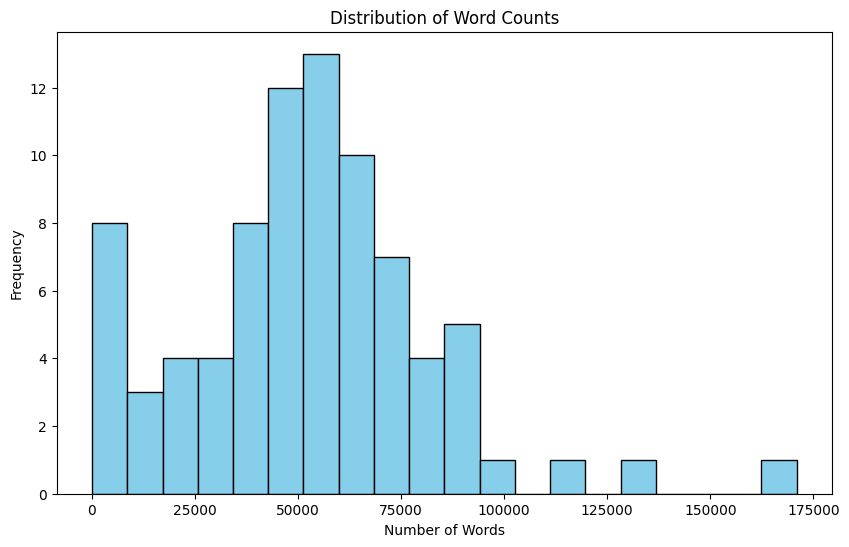
\includegraphics[width=1\textwidth]{Figures/word_distribution.png}
\caption{The size of the reports in the database}
\label{fig:word_distribution}
\end{figure}

Most reports are between 0 and 100K words long. Overall, the reports length is relatively evenly distributed: there are a few outliers (8-k reports are the smallest ones, and annual reports from the big companies are the longest).

Table \ref{table:companies} shows the list of companies, report periods and filing types that appear in the final dataset.
\begin{table}[H]
\centering
\resizebox{\textwidth}{!}{
\begin{tabular}{|c c c c|}
 \hline
 Company & Periods & Types & Total \\ [0.5ex] 
 \hline\hline
 3M & 2018, 2022, 2023Q2 & 10-K/Q & 3 \\ 
 Activision Blizzard  & 2019 & 10-K & 1 \\
 Adobe & 2015-2017, 2022  & 10-K & 4 \\
 AES Corporation & 2022 & 10-K & 1 \\
 Amazon & 2017, 2019 & 10-K & 2 \\ 
 Amcor & 2020, 2022, 2023 & 10-K/Q, 8-K & 5 \\
 AMD & 2015, 2022 & 10-K & 2 \\
 American Express & 2022 & 10-K & 1 \\
 American Water Works & 2020-2022 & 10-K & 3 \\
 Best Buy & 2017, 2019, 2023 & 10-K & 3 \\
 Block (Square) & 2016, 2020 & 10-K & 2 \\
 Boeing & 2018, 2022 & 10-K & 2 \\
 Coca-Cola & 2017, 2021, 2022 & 10-K & 3 \\
 Corning & 2020-2022 & 10-K & 3 \\
 Costco & 2021 & 10-K & 1 \\
 CVS Health & 2018, 2022 & 10-K & 2 \\
 Foot Locker & 2022 & 8-K & 2 \\
 General Mills & 2019, 2020, 2022 & 10-K & 3 \\
 Johnson\&Johnson & 2022-2023, 2022Q4, 2023Q2 & 10-K, 8-K & 4 \\
 JPMorgan & 2021Q1, 2022, 2022/23Q2 & 10-K/Q & 4 \\
 Kraft Heinz & 2019 & 10-K & 1 \\
 Lockheed Martin & 2020-2022 & 10-K & 3 \\
 MGM Resorts & 2018/20/22, 2022Q4/2023Q2 & 10-K/Q & 5 \\
 Microsoft & 2016, 2023 & 10-K & 2 \\
 Netflix & 2015, 2017 & 10-K & 2 \\
 Nike & 2018, 2019, 2021, 2023 & 10-K & 4 \\
 Paypal & 2022 & 10-K & 1 \\
 PepsiCo & 2021, 2022, 2023, 2023Q1 & 10-K, 8-K & 4 \\
 Pfizer & 2021, 2023Q2 & 10-K/Q & 2 \\
 Ulta Beauty & 2023, 2023Q4 & 10-K/Q & 2 \\
 Verizon & 2021, 2022 & 10-K & 2 \\
 Walmart & 2018-2020 & 10-K & 3 \\ 
 \hline\hline
 Total & - & - & 82 \\ [1ex] 
 \hline
\end{tabular}
}
\caption{Financial reports dataset}
\label{table:companies}
\end{table}
The annual reports have been shown to be one of the most important external documents of a company. A Form 10-K is an annual report required by the U.S. Securities and Exchange Commission (SEC), which gives a comprehensive summary of a company's financial performance \cite{USSEC.2024}. Companies with more than USD 10 million in assets and a class of equity securities that is held by more than 2000 owners must file annual and other periodic reports, regardless of whether the securities are publicly or privately traded. Following the guidance of the SEC, it should contain 4 parts and 22 Items. 

If a shareholder requests a company's Form 10-K, the company must provide a copy. In addition, most large companies must disclose on Form 10-K whether the company makes its periodic and current reports available, free of charge, on its website. Form 10-K, as well as other SEC filings may be searched at the EDGAR database on the SEC's website \cite{SECOfficeofInvestorEducationandAdvocacy.2021}.

In addition to the 10-K, which is filed annually, a company is also required to file quarterly reports on Form 10-Q. Information for the final quarter of a firm's fiscal year is included in the annual 10-K, so only three 10-Q filings are made each year. In the period between these filings, and in case of a significant event, such as a CEO departing, material cybersecurity incident or bankruptcy, a Form 8-K must be filed in order to provide up to date information \cite{SECOfficeofInvestorEducationandAdvocacy.2021}.

Laws and regulations prohibit companies from making materially false or misleading statements. Likewise, companies are prohibited from omitting material information that is needed to make the disclosure not misleading. In addition, a company’s CFO and CEO must certify to the accuracy of the 10-K and 10-Q.
The SEC does not vouch for the accuracy of a 10-K or 10-Q. The SEC sets the disclosure requirements – the topics that all companies must cover in their 10-Ks or 10-Qs, and how the information should be presented \cite{SECOfficeofInvestorEducationandAdvocacy.2021}.

The SEC staff reviews 10-Ks and 10-Qs to monitor and enhance companies’ compliance with the requirements. Both the SEC and the staff also provide interpretive advice about the disclosure requirements. The SEC staff reviews 10-Ks and may provide comments to a company where disclosures appear to be inconsistent with the disclosure requirements or deficient in explanation or clarity. The Sarbanes Oxley Act requires the SEC to review every public company’s financial statements at least once every three years. The SEC staff may review the 10-Ks and 10-Qs of certain companies more frequently \cite{SECOfficeofInvestorEducationandAdvocacy.2021}.

The length and complexity of each 10-K are company-specific, for the purposes of financial analysis and corporate valuation the following sections are where most of the time is spent: Business, Risk Factors, Management Discussion and Analysis (MDA), Financial Statements, Supplementary Disclosures. Companies are required to present their financial statements according to a set of accounting standards, conventions and rules known as Generally Accepted Accounting Principles, or GAAP. An independent accountant audits the company’s financial statements. For large companies, the independent accountant also reports on a company’s internal controls over financial reporting.


\subsection{Questions sets}
Within the framework of the present work the experiments were conducted with two lists of questions: the first list consists of 35 most common and widespread questions (for convenience we will call it Regular Questions) and the list of questions from FinanceBench dataset (FinanceBench Questions).

Regular Questions\footnote{\url{https://github.com/winterForestStump/thesis/blob/main/questions/questions_ver2.txt}} is a TXT list with 35 questions on each new line with no company names (the questions are identical for each company) regarding different topics:
\begin{enumerate}
\item Questions about the financial indicators.
\begin{itemize}
    \item The total revenue is an indicator of the overall market performance and growth: typically, a steady increase in revenue indicates healthy growth.
    \item Cost of Goods Sold (COGS) represents the direct costs attributable to the production of goods sold by the company.
    \item Gross profit margin is calculated as (Revenue - COGS) / Revenue and indicates how well the company is managing its production costs relative to its sales.
    \item Major operating expenses include selling, general, and administrative expenses, research and development costs, and other overheads.
    \item Operating income, or operating profit, reflects the company’s profitability from core operations, excluding non-operating income and expenses.
    \item Net income represents the company’s total profit after all expenses, taxes, and interest.
    \item Total outstanding debt, along with its structure and interest rates, is crucial for assessing financial risk: a well-structured debt with manageable interest rates is less risky, high levels of debt could be concerning if not matched with strong earnings.
    \item Operating cash flow is a measure of the cash generated by the company's core business activities.
\end{itemize}
\item Questions about the financial ratios. 
\begin{itemize}
    \item Earnings Per Share (EPS) measures the profitability available to each share of common stock, making it a key indicator for investors, comparing EPS with industry benchmarks provides context on the company's relative performance.
    \item Capital expenditures (CapEx) represents the company’s investment in its fixed assets, significant CapEx could indicate expansion or upgrades of facilities and equipment.
    \item The current ratio (current assets/current liabilities) and quick ratio (quick assets/current liabilities) are key indicators of the company’s short-term liquidity.
    \item Inventory levels and turnover rates provide insights into inventory management efficiency: high inventory turnover is generally favorable, indicating efficient sales and inventory management; Conversely, excess inventory may signal potential management issues.
    \item Accounts receivable turnover measures how effectively the company collects revenue: high turnover indicates efficient collection processes, while low turnover may suggest issues with credit policies or customer payment delays.
\end{itemize}
\item Questions about risks, market share, future plans and other. 
\begin{itemize}
    \item The company’s 10-K report outlines significant risks and mitigation strategies, these insights are critical for understanding potential future challenges and the company’s preparedness.
    \item Understanding the company’s market share and how it has evolved helps assess competitive positioning.
    \item The Management Discussion and Analysis (MD\&A) section provides management’s perspective on financial results, business conditions, and future outlook, it offers valuable insights into strategic priorities and operational focus.
    \item Ongoing legal proceedings can impact financial stability and reputation, understanding these issues and their potential impact is essential for risk assessment.
    \item The effective tax rate and any tax-related risks or benefits are crucial for understanding net income variability, tax strategies can significantly influence profitability.
    \item Research and Development (R\&D) spending indicates the company’s commitment to innovation: significant projects or innovations in progress can provide a competitive edge and drive future growth.
    \item Share buyback programs can signal management’s confidence in the company’s prospects. Understanding the rationale behind buybacks helps assess their impact on shareholder value.
    \item Analyzing the company's dividend history helps assess the sustainability of dividend payouts.
    \item Employee benefits and corporate culture play a significant role in attracting and retaining talent: a positive culture can drive productivity and innovation.
    \item Environmental, Social, and Governance (ESG) concerns and sustainability initiatives are increasingly important to investors and consumers.
    \item The geographic distribution of revenue provides insights into market diversification and regional performance.
    \item Managing currency risk is essential for companies operating internationally. Understanding the impact of currency fluctuations on financials helps assess economic exposure.
    \item Disclosed accounting policies and potential changes can affect financial statements.
    \item Pension obligations and contributions are important for assessing long-term financial commitments: a pension fund surplus or deficit can significantly impact financial health.
    \item Leveraging technology for operations and ongoing advancements can enhance efficiency and competitiveness.
    \item Management’s views on future growth, strategic plans, and anticipated challenges provide a road map for potential developments and market positioning.
\end{itemize}
\end{enumerate}

The second set of questions is FinanceBench Questions\footnote{\url{https://github.com/patronus-ai/financebench/blob/main/data/financebench_open_source.jsonl}}, which consists of 150 specific to the each company questions with provided ground truth answers. The questions collected are realistic and applicable to real-world financial scenarios and include complex questions that require computational reasoning to arrive at conclusive answers.


\subsection{Experiments Setup}
Google Disk (free subscription) was used to store the reports and vector database. Since executing code on CPU is very slow (some operations are 18 times slower on CPU then GPU) and using the Google virtual machine Colab Free Tier is almost impossible due to time and GPU usage limits. A monthly Google Colab Pro subscription (EUR 11.01 with VAT) was purchased, which provides a virtual machine with 100 computational units (usage rate is approximately 1.76 per hour for T4 GPU), 12.7GB system RAM, 15GB GPU RAM and 201.2GB Disk Storage.

Open-sourse libraries and frameforks were used, no API was used. HuggingFace\footnote{https://huggingface.co/} was used to access embeddings models and LLMs. The LLamaCpp\footnote{https://github.com/ggerganov/llama.cpp} framework was also used to inference with Meta's LLAMA architecture model locally. The LangChain\footnote{\url{https://https://github.com/langchain-ai/langchain/}} framework was used for creating RAG architecture with retrievals and chains.

\subsection{Database Deployment}
Annual reports are unstructured data, they cannot be stored in a pre-defined format or fit into an existing data (table-based) model. For tokenization (creating vector representation of the text) annual reports the "BAAI/bge-small-en-v1.5" embedding model from HuggingFace was used. The vectors were normalized to calculate cosine similarity between them.

Since reports are long, they should be divided into parts. For chunking 'RecursiveCharacterTextSplitter' (from LangChain library) was used. It tries to split on the default list of characters in order until the chunks are small enough. This has the effect of trying to keep all paragraphs (and then sentences, and then words) together as long as possible, as those would generically seem to be the strongest semantically related pieces of text. The number of characters in each chunk (chunk size) is 256. The LangChain library offers many other different types of text splitters: HTML splits on html specific characters, Markdown - on markdon specific characters and others. At a high level, text splitters work as following: Split the text up into small, semantically meaningful chunks (often sentences). Start combining these small chunks into a larger chunk until you reach a certain size (as measured by some function). Once you reach that size, make that chunk its own piece of text and then start creating a new chunk of text with some overlap (to keep context between chunks)\footnote{\url{https://python.langchain.com/v0.1/docs/modules/data_connection/document_transformers/}}.

The choice of the correct chunk size is not a trivial task. Firstly, there is a limitation from the maximum sequence length of the embedding model. Since bge-small-en-v1.5 model basis on BERT than the maximum sequence length is 512, so the maximum chunk size should be less than 512. Otherwise, the model applies a truncation strategy and silently ignores all tokens after 512 one. There is a trade off between 128, 256 or 512 sizes between preserving context and maintaining accuracy. Smaller chunks may provide better accuracy but lost context. The best way is by exploring a variety of chunk sizes, including smaller chunks (e.g., 128 or 256 tokens) for capturing more granular semantic information and larger chunks (e.g., 512 or 1024 tokens) for retaining more context. But that wasn't in the scope of our paper. In order to maintain a balance between preserving context and accuracy we decided to use a  'ParentDocumentRetriever' (from LangChain library). The 'ParentDocumentRetriever' splitts and storing small chunks of data (child chunks). During retrieval, it first fetches the small chunks but then looks up the parent ids for those chunks and returns those larger documents (parent chunks). For child chunk we have chosen the size of 256 tokens (for the accuracy) and for the parent chunks the size of 2000 (to preserve the context). 

For storing vector embeddings we use collections in ChromaDB. We have created 3 collections with the same vector, but with different distance functions: euclidean distance (l2), inner product, cosine similarity. ChromaDB uses distance function to search through the database and compute the similarity. Our first experiments are about to compare all 3 functions and choise the best one to work with in future. 

After the collections were created we used a JSONLoader (from LangChain library) to load reports in JSON format. While loading we also define the metadata for every chunk with some useful information such as CIK, company name, filing type and date, period of report, state location, fiscal tear end, html filing link and filename. We will use company name in future experiments for filtering queries during the database search stage. All other metadata keys may also be used in future to enhance retrieval part of the system.

In total there are 17561 parent chunks which are divided into 356275 child chunks, which are stored in every collection in the Chroma database. Estimated storage for every collection can be calculated by formula \cite{QuentinAnthonyStellaBidermanHaileySchoelkopf.2023}: Storage = Dimensionality of the vectors x 4 bytes x Number of documents (chunks).

384 (dimension of the vectors) x 4 (bytes) x 356275 (chunks) = 547 Mb. Every collection additionally has ids, metadata and indexes.


\subsection{Initial Experiments with RAG Architectures}
In this section the results of the first experiments with different RAG architectures are provided. Some of the conclusions from the experiments will be used in the following subsections.

Using the embedding model the report's texts were tokenized into vectors, splitted with 'RecursiveCharacterTextSplitter' into small (256 tokens) and big (2000 tokens) chunks and stored into the ChromaDB collection with a default Euclidean distance function. Questions from the Regular Questions were asked about 5 companies (Nike, CocaCola, 3M, Adobe, General Mills). Each question was augmented with the company's name. 'ParentDocumentRetriever' searched for the most similar chunks to the questions in the database and returned them as the context to the LLM.

For answering the questions Llama-2-7b-Chat-GPTQ model from HuggingFace was used\footnote{\url{https://huggingface.co/TheBloke/Llama-2-7B-Chat-GPTQ}}. Llama 2 is an auto-regressive language model that uses an optimized transformer architecture, was trained between January 2023 and July 2023. The model had following hyper-parameters: temperature (controls randomness of predictions; for use cases that need to always be factually grounded, very low temperature values are recommended, while more creative tasks can benefit from higher temperatures.) = 0.0001, max\_new\_tokens (number of generated tokens) = 2048, top\_p (manages randomness) = 0.9, repetition\_penalty (discourages repetitive or redundant output) = 1.1. The model after receiving the retrieved documents as context, provided responses for every question\footnote{\url{https://github.com/winterForestStump/thesis/blob/main/notebooks/experiment_llama2_chain_filter_flashrerank.ipynb}}. 

The LLM's system prompt for the model was the following: "Use the following information from company annual reports and answer the question at the end. If the answer is not contained in the provided information or if there is NO context at all, say "The answer is not in the context". 

The responses were manually evaluated. Two binary questions were asked to each question-answer pairs: 'Is the context relevant to the company?" and "Is the context relevant to the question?" to to assess the quality of the system retrieval process. The answers to the questions are binary - 'Yes' and 'No'. Each 'Yes' answer corresponds to 1, and each 'No' answer corresponds to 0. Later, all results for each question are summed and the usual average is calculated: (number of positive answers)/ (total number of answers).

Experiments were conducted with the following architectures: 1) Naive (simple) RAG and 2) Naive RAG plus metadata filtering during the retrieval stage, when company's name was provided for the search filter to the 'ParentDocumentRetriever':
\begin{verbatim}
search_kwargs = {'filter': {'company': COMPANY_NAME}}
\end{verbatim}
The results of the experiments are shown in the \autoref{table:initial}.\\ 

\begin{table}[h!]
\centering
\resizebox{\textwidth}{!}{
\begin{tabular}{|c|c|c|}
\hline
Metric & Naive & Naive + Filter \\ [0.5ex] 
\hline
Is the context relevant to the company? & 0.743 & 1.000 \\ 
Is the context relevant to the question?  & 0.600 & 0.657 \\[1ex] 
\hline
\end{tabular}
}
\caption{Results of the initial experiments}
\label{table:initial}
\end{table}

The initial experiments with different Retrieval-Augmented Generation (RAG) architectures yielded several key insights that will inform future analysis:
\begin{enumerate}
\item Using a company name filter significantly improved the relevance of the retrieved context to the company, achieving 100\% accuracy. This approach also enhanced the context's relevance to the question, increasing the score from 0.600 to 0.657.
\item For effective filtering, it is crucial to use the exact company name as specified in the metadata. This ensures precise and relevant document retrieval.
\item The retrieval process did not incorporate date filtering, resulting in the retrieval of identical chunks from documents across different dates. This suggests that date-specific relevance was not considered in the initial experiments.
\item The responses generated by the Llama-2-7b-Chat-GPTQ model were noted to be unstable and unpredictable, indicating a need for further refinement in handling the retrieved context.
\item The results are based on experiments conducted with five companies (Nike, CocaCola, 3M, Adobe, General Mills). Therefore, additional testing with a broader range of companies is necessary to generalize the findings.
\end{enumerate}

For future experiments, applying metadata filtering is essential to maintain high relevance and accuracy. 

\subsection{Retrieval Experiments}
\subsubsection{Distance Functions}
There are three primary distance functions: L2 or Euclidean distance, cosine similarity, and inner product, which can be used by a database for similarity search in vector storage.  The question of using different functions depends on the nature of the data and the task at hand.

Euclidean distance is primarily used when the magnitudes of the vectors differ, and the primary concern is the actual distance or semantic distance between words in space. In contrast, cosine similarity focuses on the difference in semantic orientation between vectors. When vectors are normalized, cosine similarity becomes equivalent to the inner product. The inner product itself combines aspects of both Euclidean distance and cosine similarity. It is faster than cosine similarity and offers greater flexibility.

The mathematical formulas for different distance functions are in the \autoref{table:formulas}.
\begin{table}[h!]
\renewcommand{\arraystretch}{2.5}
\centering
\begin{tabular}{|>{\centering\arraybackslash}m{4cm}|>{\centering\arraybackslash}m{9cm}|}
\hline
\textbf{Measure} & \textbf{Formula} \\ \hline
\textbf{Euclidean Distance} & \( d(\mathbf{a}, \mathbf{b}) = \sqrt{\sum_{i=1}^{n} (a_i - b_i)^2} \) \\ \hline
\textbf{Inner Product} & \( \mathbf{a} \cdot \mathbf{b} = \sum_{i=1}^{n} a_i b_i \) \\ \hline
\textbf{Cosine Similarity} & \( \cos(\theta) = \frac{\sum_{i=1}^{n} a_i b_i}{\sqrt{\sum_{i=1}^{n} a_i^2} \sqrt{\sum_{i=1}^{n} b_i^2}} \) \\ \hline
\end{tabular}
\caption{Distance Functions Formulas}
\label{table:formulas}
\end{table}

Distance function for the collection in ChromaDB cannot be changed after the collection is created. In order to chose the best distance function to use, the experiments were conducted on 3 identical collections of vectors (embedded chunks of financial reports) with 3 different distance functions.

In preparing the experiments, an issue arose about the wording of the questions, namely the need to use the company name in the question. Intuitively, realizing that not every chunk contains the name of the company of interest, and the use of the company name in the question may worsen the quality of the semantic search. But for the final decision, it was decided to experiment with two approaches:
\begin{enumerate}
\item The first approach does NOT include the company name in the question;
\item The second approach is that each question contains the company name.
\end{enumerate}

During the experiments 35 questions from the Regular Questions set were asked to the 3 collections (with different distance functions: cosine similarity, inner product, l2) about 13 random companies from the database deployed ('COCA COLA CO', 'AMAZON COM INC', 'PayPal Holdings, Inc.', 'GENERAL MILLS INC', 'Walmart Inc.', 'PEPSICO INC', 'Kraft Heinz Co', 'Amcor plc', 'Square, Inc.', '3M CO', 'MICROSOFT CORP', 'Ulta Beauty, Inc.', 'AES CORP') in one run with 2 approaches (with company name in the question and without). In total 78 (2 approaches x 13 companies x 3 distance functions) retrieval runs\footnote{\url{https://github.com/winterForestStump/thesis/blob/main/retrieval/Retrievals_approaches.ipynb}} were conducted. Every run provides 70 question-context pairs: 2 the most relevant parent chunks to each of 35 questions, saved as JSON files\footnote{\url{https://github.com/winterForestStump/thesis/tree/main/retrieval/retrievals}}.

To evaluate the results of the retrievals the "Phi-3-mini-4k-instruct-fp16.gguf" model was utilized, a GGUF format for the Phi-3-Mini-4K-Instruct model from Microsoft. The GGUF\footnote{\url{https://github.com/ggerganov/ggml/blob/master/docs/gguf.md}} format is specially designed to store inference models and perform well on consumer-grade computer hardware. 

To run the model locally the LLamaCpp with temperature (is used to control the generation randomness) equals 0 and context window (the maximum number of context tokens) equals 4096 was utilized. The model was provided with question and the retrieved context for every approach and distance function and was asked to evaluate the relevance. For each approach, the prompt templates differed only in the input variable names: approach 1 does not include the company name in the question, and the input variable name is 'question'; approach 2 includes the company name in the question, and the input variable name is 'question\_name'. 

The assistant part of the prompt is the same for both approaches: "You are a grader assessing relevance of a retrieved document to a user question. If the document contains keywords related to the user question, grade it as relevant. It does not need to be a stringent test. The goal is to filter out erroneous retrievals. Give a binary score 'yes' or 'no' score to indicate whether the document is relevant to the question. Provide the binary score as a JSON with a single key 'score' and no preamble or explanation."

For every question-document pair, the model provided binary answers: 'Yes' if the document contains information relevant to the question, or 'No' if the document does not contain information related to the question. The final score was calculated as an average from the model's responses: (Total number of "Yes" answers) / (Total number of all answers). The average similarity score was calculated for each approach and distance function\footnote{\url{https://github.com/winterForestStump/thesis/blob/main/retrieval/Retrievals_approaches_evaluation_phi3.ipynb}}.

The final results are presented in the table. The average score for every approach is in fact a precision (the fraction of relevant instances among the all retrieved instances): 
\[
\text{Precision} = \frac{\#(\text{relevant items retrieved})}{\#(\text{retrieved items})} = P(\text{relevant} \mid \text{retrieved})
\]

It is impossible to calculate recall, which is the fraction of relevant instances that were retrieved, due to the unlabeled dataset and the absence of ground truth context.

The final results for both approaches and all of the distance functions are in the \autoref{table:scores}:\\
\begin{table}[h!]
\renewcommand{\arraystretch}{2.5}
\centering
\begin{tabular}{|>{\centering\arraybackslash}m{4cm}|>{\centering\arraybackslash}m{3cm}|>{\centering\arraybackslash}m{3cm}|}
\hline
\textbf{Measure} & \textbf{Approach 1} & \textbf{Approach 2}\\ \hline
\text{Euclidean Distance} & \textbf{0.5723} & 0.3688 \\ \hline
\text{Inner Product} & 0.5671 & 0.3571 \\ \hline
\text{Cosine Similarity} & 0.5716 & 0.3794 \\ \hline
\end{tabular}
\caption{Average scores for different approaches and distance functions}
\label{table:scores}
\end{table}

Approach 1, without mentioning the company name in the questions, shows significantly better results. This confirms the initial intuition that not every small (or even large) text chunk contains a mention of the company name, which makes the question and the text part closer in meaning (with a better similarity coefficient). 

The average scores of distance functions in different approaches are quite close to each other, but the best result is Eucleadian Dicstance (L2). 

Important to note, that in the experiments the normalized data was used. The results of some researches demonstrate that the normalization of the full dataset, may lead to biased results, surprisingly, for the worse, and Euclidean distance showed not the best results \cite{Barboza.30Jun2023}.

To further analyze which questions caused the most difficulty in the document retrieval phase, the Approach 1 data for all three distance functions ere analyzed together (since they showed nearly identical results) for each of the 35 questions\footnote{\url{https://github.com/winterForestStump/thesis/blob/main/retrieval/approach_1_combined_analysis.ipynb}}:
\newcolumntype{L}[1]{>{\raggedright\arraybackslash}p{#1}}
\begin{longtable}{L{0.6\textwidth}rrr}
\toprule
question & total & correct & percentage,\% \\
\midrule
\endfirsthead
\toprule
question & total & correct & percentage,\% \\
\midrule
\endhead
\midrule
\endfoot
\endlastfoot
What does the company foresee in terms of future growth and challenges and are there any strategic plans outlined for the upcoming years? & 74 & 71 & 95 \\
What is the effective tax rate for the company? & 73 & 70 & 95 \\
Are there any ongoing legal proceedings against the company? & 73 & 68 & 93 \\
What is the company's operating income and how does it compare to the previous years? & 68 & 61 & 89 \\
What potential impact could legal issues have on the business of the company? & 77 & 69 & 89 \\
Are there any tax-related risks or benefits for the company mentioned? & 75 & 66 & 88 \\
Who are the company's main competitors and how does the company differentiate itself? & 66 & 56 & 84 \\
How does the company manage currency risk and are there impacts on financials due to currency fluctuations? & 71 & 58 & 81 \\
What is the total revenue generated by the company and how has the revenue changed over the past few years? & 67 & 54 & 80 \\
What are the company's critical accounting policies disclosed and how might changes in these policies affect financial statements? & 70 & 56 & 80 \\
How does the company's management view the company performance? & 70 & 55 & 78 \\
What is the company's cash flow generated from operations and are there any notable trends or fluctuations? & 69 & 54 & 78 \\
Has the company engaged in any share buyback programs and if yes what is the rationale behind such actions? & 68 & 53 & 77 \\
What is the company's net income for the current fiscal year and how has net income trended over the past few years? & 72 & 53 & 73 \\
What employee benefits does the company offer? & 71 & 52 & 73 \\
What are the company's key risks mentioned in the 10-K and how does the company plan to mitigate these risks? & 66 & 46 & 69 \\
What are the company's major operating expenses and how have these expenses changed over time? & 75 & 50 & 66 \\
How much has the company invested in capital expenditures and are there any significant projects underway? & 68 & 43 & 63 \\
How does the company leverage technology for its operations and are there ongoing technological advancements? & 70 & 43 & 61 \\
What is the company's geographic breakdown of revenue and are there any notable trends or shifts? & 76 & 44 & 57 \\
How does the company address Environmental, Social, and Governance (ESG) concerns and are there any sustainability initiatives in place? & 72 & 41 & 56 \\
What is the company's total outstanding debt, how is the debt structured, and what are the interest rates? & 76 & 43 & 56 \\
What are the company's key insights provided in the Management Discussion and Analysis (MD\&A) section? & 71 & 39 & 54 \\
What are the company's pension obligations and contributions and is there a pension fund surplus or deficit? & 76 & 40 & 52 \\
How much is spent on research and development by the company? & 72 & 31 & 43 \\
What is the company's dividend history and how sustainable are the dividend payouts? & 76 & 30 & 39 \\
What is the company's gross profit margin, and how has it evolved? & 72 & 21 & 29 \\
What innovations or projects are currently in progress in the company? & 72 & 21 & 29 \\
How much inventory does the company hold and are there any signs of inventory management issues? & 68 & 18 & 26 \\
What is the company's cost of goods sold (COGS) and how does the COGS compare to the total revenue? & 70 & 11 & 15 \\
What is the company's earnings per share and how does it compare to industry benchmarks? & 77 & 10 & 12 \\
How is the company's corporate culture described? & 77 & 8 & 10 \\
What is the company's market share in its industry and how has it changed over the years? & 78 & 4 & 5 \\
What is the company's accounts receivable turnover and are there any concerns regarding receivables aging? & 64 & 1 & 1 \\
What is the company's current ratio and quick ratio and how do these ratios compare to industry averages? & 70 & 0 & 0 \\
\hline
Total & 2510 & 1440 & 57 \\
\hline
\caption{The results for Approach 1 and for all 3 distance metrics} \\
\end{longtable}

The 'total' number is the number of retrieved context from the ChromaDB using the similarity scores, the 'correct' number shows the number of times when the LLM answered that the provided context is relevant to the question. The 'percentage' column is an average score, showing the accuracy. The maximum number of "total" number is 78 (2 the most relevant chunks x 13 companies x 3 distance functions). Approach 1 received a total of 2510 question-answer-evaluation pairs, this is less than 2,730 (78 x 35 questions) because not always two the most similar chunks were received for each question, but sometimes for some questions only one, and because of 15 evaluation errors. 

Based on the data presented in the table, we can draw several conclusions and inferences about the effectiveness of document retrieval according to the given questions:
\begin{enumerate}
\item Questions related to future growth, challenges, strategic plans, and effective tax rates exhibit high accuracy (95\%). This suggests that these types of information are clearly and consistently presented in documents, making them easier to retrieve accurately.
\item Questions about legal proceedings, operating income, and potential legal impacts also have high accuracy (89-93\%). Legal data seems to be well-documented in company reports, aiding retrieval accuracy.
\item Questions on employee benefits and key risks show lower accuracy (69-73\%). These topics may be detailed in various sections or be subject to more interpretative reporting, complicating accurate retrieval. 
\item Questions about operating expenses and capital expenditures have about 63-66\% accuracy. This suggests variability in how these figures are reported or labeled in documents.
\item Questions about the geographic breakdown of revenue, ESG initiatives, pension obligations and R\&D spending have relatively low accuracy (43-57\%). These topics may not be covered comprehensively in standard financial documents, leading to difficulty in retrieval.
\item Questions about dividend history and gross profit margin exhibit very low accuracy (29-39\%). These details can be scattered or calculated differently, challenging straightforward retrieval.
\item Questions on ongoing innovations, inventory management, and cost of goods sold (COGS) show poor retrieval performance (15-29\%). These topics often involve specific details that may not be explicitly outlined in main sections.
\item Questions regarding earnings per share, corporate culture, and market share are highly inaccurate (5-12\%). These topics might not be directly addressed in standard documents or require a level of analysis not easily retrievable through basic similarity metrics.
\item Questions on current and quick ratios, and accounts receivable turnover show near-zero accuracy (0-1\%). Such financial metrics may just absent in most of the reports, they require calculation from multiple financial sections, which is difficult with simple retrieval approaches.
\end{enumerate}

\subsubsection{Re-Ranker}
Up to this point, we've employed an embedding model to locate the top 2 relevant chunks within the database. We've kept the number of chunks (top\_k) small due to the limited context length of the LLM. However, this approach assumes that the top 2 retrieved chunks are the most relevant and correctly ordered. But the problem may arise when some relevant chunks are ranked much lower than others. In this section, we introduce re-ranking. This allows us to broaden our search within the database by retrieving more segments (top\_k = 10) and then reorder them based on the highest 2 ranking scores.

In the next stage of the analysis, for the best approach 1 and Eucleadian distance (l2) distance function, we conducted retrieval experiments with using a re-ranker - BAAI/bge-reranker-v2-m3. Different from embedding model, re-ranker uses question and document as input and directly output similarity instead of embedding. We asked the system the same 35 questions according to the approach 1 (without company names in the question) about the same 13 companies. But now 'ParentDocumentRetriever' retrieved top 10 documents (top\k = 10) and after that Re-ranker recomputed the scores and leave only 2 the best of them with the highest similarity score\footnote{\url{https://github.com/winterForestStump/thesis/blob/main/retrieval/Retrievals_l2_with_reranker.ipynb}}. Again, as in the previous experiments the company names were directly putted into the search filter of the database. As a result we have 13 JSON files with the question-content pairs\footnote{\url{https://github.com/winterForestStump/thesis/tree/main/retrieval/retrievals/reranked}}.

After we conducted the same as before evaluation of the retrieved documents relevance to the question with using "Phi-3-mini-4k-instruct-fp16.gguf" model and calculated the average score (number of 'Yes' answers divided by the number of total question-answers pairs)\footnote{\url{https://github.com/winterForestStump/thesis/blob/main/retrieval/Retrievals_reranked_l2_evaluation_phi3.ipynb}}.

The results from the \autoref{table:results} show the significant improvement in relevance of the context to the question with the average score of 0.7305.
\begin{table}[H]
\renewcommand{\arraystretch}{2.5}
\centering
\begin{tabular}{|>{\centering\arraybackslash}m{4cm}|>{\centering\arraybackslash}m{3cm}|>{\centering\arraybackslash}m{3cm}|}
\hline
\textbf{Measure} & \textbf{Naive} & \textbf{Re-Ranker}\\ \hline
\text{L2, Approach 1} & 0.5723 & \textbf{0.7305} \\ \hline
\end{tabular}
\caption{Comparison of the results without and with using Re-ranker}
\label{table:results}
\end{table}

In order to further analyze how the re-ranker influenced to the particular questions we present the data for Approach 1 Euclidean Distance with Re-ranker\footnote{\url{https://github.com/winterForestStump/thesis/blob/main/retrieval/reranker_combined_analysis.ipynb}}:

\newcolumntype{L}[1]{>{\raggedright\arraybackslash}p{#1}}
\begin{longtable}{L{0.6\textwidth}rrr}
\toprule
question & total & correct & percentage,\% \\
\midrule
\endfirsthead
\toprule
question & total & correct & percentage,\% \\
\midrule
\endhead
\midrule
\endfoot
\endlastfoot
Are there any ongoing legal proceedings against the company? & 10 & 10 & 100 \\
Are there any tax-related risks or benefits for the company mentioned? & 10 & 10 & 100 \\
What is the company's cash flow generated from operations and are there any notable trends or fluctuations? & 8 & 8 & 100 \\
What is the company's cost of goods sold (COGS) and how does the COGS compare to the total revenue? & 2 & 2 & 100 \\
What is the company's geographic breakdown of revenue and are there any notable trends or shifts? & 4 & 4 & 100 \\
What are the company's critical accounting policies disclosed and how might changes in these policies affect financial statements? & 13 & 13 & 100 \\
What is the company's operating income and how does it compare to the previous years? & 7 & 7 & 100 \\
What is the effective tax rate for the company? & 8 & 8 & 100 \\
What is the total revenue generated by the company and how has the revenue changed over the past few years? & 10 & 10 & 100 \\
What potential impact could legal issues have on the business of the company? & 13 & 13 & 100 \\
What does the company foresee in terms of future growth and challenges and are there any strategic plans outlined for the upcoming years? & 13 & 13 & 100 \\
How does the company manage currency risk and are there impacts on financials due to currency fluctuations? & 12 & 11 & 91 \\
Has the company engaged in any share buyback programs and if yes what is the rationale behind such actions? & 12 & 11 & 91 \\
What is the company's total outstanding debt, how is the debt structured, and what are the interest rates? & 7 & 6 & 85 \\
How does the company's management view the company performance? & 12 & 10 & 83 \\
How does the company leverage technology for its operations and are there ongoing technological advancements? & 11 & 9 & 81 \\
What is the company's net income for the current fiscal year and how has net income trended over the past few years? & 5 & 4 & 80 \\
Who are the company's main competitors and how does the company differentiate itself? & 10 & 8 & 80 \\
How much has the company invested in capital expenditures and are there any significant projects underway? & 9 & 7 & 77 \\
What employee benefits does the company offer? & 13 & 10 & 76 \\
What are the company's major operating expenses and how have these expenses changed over time? & 11 & 8 & 72 \\
What are the company's pension obligations and contributions and is there a pension fund surplus or deficit? & 7 & 5 & 71 \\
What are the company's key risks mentioned in the 10-K and how does the company plan to mitigate these risks? & 10 & 7 & 70 \\
What are the company's key insights provided in the Management Discussion and Analysis (MD\&A) section? & 13 & 9 & 69 \\
How much inventory does the company hold and are there any signs of inventory management issues? & 9 & 6 & 66 \\
What is the company's dividend history and how sustainable are the dividend payouts? & 11 & 7 & 63 \\
What innovations or projects are currently in progress in the company? & 13 & 8 & 61 \\
How does the company address Environmental, Social, and Governance (ESG) concerns and are there any sustainability initiatives in place? & 12 & 7 & 58 \\
How much is spent on research and development by the company? & 11 & 5 & 45 \\
What is the company's gross profit margin, and how has it evolved? & 11 & 4 & 36 \\
What is the company's earnings per share and how does it compare to industry benchmarks? & 4 & 1 & 25 \\
How is the company's corporate culture described? & 9 & 2 & 22 \\
What is the company's market share in its industry and how has it changed over the years? & 11 & 1 & 9 \\
What is the company's accounts receivable turnover and are there any concerns regarding receivables aging? & 7 & 0 & 0 \\
What is the company's current ratio and quick ratio and how do these ratios compare to industry averages? & 6 & 0 & 0 \\
\hline
Total & 334 & 244 & 73 \\
\hline
\caption{The results for Approach 1, Euclidean distance function and Re-ranker} \\
\end{longtable}

The 'total' number is the number of retrieved context from the ChromaDB using the similarity scores from the re-ranker, the 'correct' number shows the number of times when the LLM answered that the provided context is relevant to the question. The 'percentage' column is an average score, showing the accuracy.

Based on the provided experiments and analysis, we can draw several conclusions regarding the document retrieval performance for the given questions after using a re-ranker:
\begin{enumerate}
\item The use of the re-ranker significantly improved the overall accuracy of context relevance to questions, increasing from 57\% to 73\%. This suggests that the re-ranker effectively identifies the most relevant documents, enhancing the retrieval quality.
\item The re-ranker achieved perfect accuracy for several questions, including those about ongoing legal proceedings, tax-related risks, cash flow trends, cost of goods sold (COGS), geographic revenue breakdown, critical accounting policies, operating income, effective tax rate, total revenue, potential legal impacts, and future growth and challenges. 
\item Questions on currency risk management, share buyback programs, total outstanding debt, and management views achieved 83-91\% accuracy. These topics, while slightly more complex, are still well-captured by the re-ranker, demonstrating its effectiveness in handling moderately complex information.
\item Questions regarding technology leverage, net income trends, main competitors, capital expenditures, employee benefits, major operating expenses, pension obligations, key risks, and MD\&A insights show accuracy between 70-80\%. These topics may involve a mix of quantitative data and qualitative analysis, making them moderately challenging but still manageable for the re-ranker.
\item Questions about inventory management, dividend history, ongoing innovations, and ESG concerns have accuracy between 58-66\%. These areas often involve diverse and less standardized information, posing challenges for accurate retrieval.
\item Research and development (R\&D) spending, gross profit margin, and earnings per share questions show low accuracy (25-45\%). These metrics may not be prominently featured or might require detailed extraction and contextual understanding, which the re-ranker struggles with.
\item Questions about corporate culture, market share, accounts receivable turnover, and financial ratios (current and quick ratios) exhibit very low to no accuracy (0-25\%). These topics may not be directly addressed in documents or require synthesis of dispersed information, highlighting limitations in the re-ranker’s current capabilities.
\item The significant improvement in overall accuracy underscores the effectiveness of re-rankers in refining document retrieval processes. By prioritizing the most relevant documents, re-rankers enhance the relevance and precision of the information retrieved.
\item The highest accuracy is achieved for questions involving standardized financial and strategic information. Conversely, complex or less standardized data, such as cultural insights or detailed financial ratios, remain challenging.
\item The variability in accuracy for different types of questions indicates that the structure and comprehensiveness of company documents play a significant role in retrieval success. Improving document indexing and section-specific retrieval methods could further enhance performance.
\end{enumerate}

Euclidean distance function will be used in further experiments as the underlying distance measure.

\subsection{RAG Experiments}
\subsubsection{Experiments Methodology}
Using the results from the previous experiments to create a better RAG pipeline architecture, four experiment configurations were conducted in total:
\begin{enumerate}
\item Regular Questions set using RAG pipeline\footnote{\url{https://github.com/winterForestStump/thesis/blob/main/notebooks/rag_x_phi3_generalQA.ipynb}};
\item Regular Questions set without using RAG pipeline, a baseline without using retrieval part, questions are asked to the model without providing additional context (No RAG)\footnote{\url{https://github.com/winterForestStump/thesis/blob/main/notebooks/noRag_x_phi3_generalQA.ipynb}};
\item FinanceBench Questions set using RAG pipeline\footnote{\url{https://github.com/winterForestStump/thesis/blob/main/notebooks/rag_x_phi3_financebenchQA.ipynb}};
\item FinanceBench Questions set without using RAG pipeline, a baseline without using retrieval part (No RAG)\footnote{\url{https://github.com/winterForestStump/thesis/blob/main/notebooks/noRag_x_phi3_financebenchQA.ipynb}}.
\end{enumerate}

The questions from Regular Questions set were asked about the following companies: 3M, Amazon, Coca-Cola, JPMorgan Chase, Locheed Martin, Microsoft, Nike, PayPal, Verizon Communications, Walmart. The results for every company were saved as JSON files\footnote{\url{https://github.com/winterForestStump/thesis/tree/main/evaluation}}. Experiments with using RAG starts with using model to convert the company's name into the correct spelling. The user can enter the name in any way, the model convert it to the precise name from the metadata list, this is essential because the company's name is used in searching filtering in database. After the retriever is searching the most 20 similar chunks in the database, which will be re-ranked into the 2 the best fit chunks. Next, the question (tokenized with the same embedding model as all the reports in the database) and chunks are fed as context to the model. Regular Questions do not specify specific dates of interest, i.e. the system can provide data for any period.

Experiments without using RAG pipeline, a baseline without using retrieval part, (No RAG) were conducted without providing the model any additional information related to the question from the database as context. In fact, the experiments tested the internal knowledge of the model, fixed in its parameters. Regular Questions have been changed and company names have been added to the questions.

Important to note that for FinanceBench Questions the company name is not reliably extracted by the model (apparently the model is too small for this). An experiment \footnote{\url{https://github.com/winterForestStump/thesis/blob/main/notebooks/rag_x_phi3_financebenchQA.ipynb}} using the Phi-3 model to extract company names from the questions showed an accuracy of only 72\%\footnote{\url{https://github.com/winterForestStump/thesis/blob/main/evaluation/financebench150/questions_metadata_names_retrieved.ipynb}}. Therefore the company name for each question was manually entered into the database search filter. Without this, the quality of search, retrieval and as a consequence the answer to the question would have been even worse.

The main goals of the experiments are to evaluate the results of the RAG chain and to measure the improvement RAG provides, comparing results from RAG and No Rag settings. To evaluate the results of the experiments, a human evaluation was conducted.

\subsubsection{Experiments Limitations}
\begin{enumerate}
\item The company name filter was set manually as a SQL filter in the vector database:
\begin{verbatim}
search_kwargs = {'filter': {'company': COMPANY_NAME}}
\end{verbatim}
This approach was necessary because the language model is not stable and reliable in determining the correct company name from the question (the accuracy of using Phi-3-mini model is 72\%). For general QA questions, no hard filter on dates of interest was specified, as these questions do not relate to any particular time period.
\item Since dates are not strictly set in the filter or the question, two identical (or very similar) blocks of text and data for different time intervals may be retrieved at the retrieval stage. In this case, the model selects data for later dates. For example, if the context contains data for 2015 and 2022, the model will use 2022 data to generate the answer.
\item A large number of responses contain general information, making it difficult to assess the extent to which the model utilized the provided context versus its own knowledge. Notably, many answers with specific meanings are incorrect.
\item Although the Phi-3 model's technical documentation specifies a cutoff period of October 2023 for model training, most of the model's non-RAG responses reference data from 2020 and 2021.
\item The process of evaluating is extremely subjective. Maintaining consistency in metrics is difficult due to the variety of information requested and the complexity of the data in the reports. The evaluation process was conducted by a single evaluator, which could lead to mistakes due to inattention or lack of knowledge.
\item Even if the retrieved document (context) is relevant to the question and the model provides a useful result, the answer is often incomplete due to limitations in the context size (2k tokens each) and the model's context window (4k tokens). This is insufficient for most questions, making it virtually impossible to reliably understand and assess the completeness and comprehensiveness of the response. It is clear that the responses are incomplete and there is a high probability of missing important information.
\item Some answers are well-formed paraphrases or summaries of the context. While the answers may contain many key words and phrases, they are often not specific enough to be useful to the user. This may be a reason for the problematic evaluation of results with LLM.
\end{enumerate}


\subsubsection{Evaluation and Results for the Regular Questions set}
For the Regular Questions set the questions, retrieved context (whether relevant or irrelevant to the question), and generated responses were saved as a CSV file. This dataset was then uploaded to the Argilla workspace (a framework that utilizes HuggingFace space) for manual annotation. The dataset was evaluated using the following metrics, with set of ["YES", "NO", "UNSURE"] possible answers for each question:
\begin{enumerate}
\item Relevancy metric. The answer to the question "Are the retrieved documents relevant to the given question?"
\item Faithfulness metric. The answer to the question "Is the generated answer grounded in/supported by the context (retrieved documents)?". If it was not possible to verify the data from a response within a reasonable time frame, the "faithfulness" metric was assigned a value of "UNSURE".
\item Usefulness metric. The answer to the question "Is the generated answer useful in resolving the question?". If the answer is incorrect or irrelevant, it is not useful. If the response merely indicates where the requested data can be obtained, it is considered unhelpful. A 'YES' for the 'usefulness' metric indicates correct answers or answers containing some correct information. 'NO' also includes factually incorrect answers and responses where the context does not contain relevant information, and the LLM's answer is simply "I do not know" or "I do not have specific information".
\end{enumerate}

After all the results of the experiments with Regular Questions set were evaluated on Argilla workspace, the results were analyzed. The distribution of responses between the metrics is shown in the \autoref{table:comparison_RA}:
\begin{table}[h]
\centering
\begin{tabular}{|c|c|c|c|c|}
\hline
\textbf{Metric} & \textbf{Setup} & \textbf{YES} & \textbf{UNSURE} & \textbf{NO} \\ 
\hline
\multirow{2}{*}{Relevancy} & No RAG & 0 (0\%) & 0 (0\%) & 0 (0\%) \\ \cline{2-5}
 & RAG & 208 (60\%) & 30 (9\%) & 109 (31\%) \\
\hline
\multirow{2}{*}{Faithfulness} & No RAG & 75 (21\%) & 190 (54\%) & 85 (24\%) \\ \cline{2-5}
 & RAG & 317 (91\%) & 1 (0\%) & 29 (8\%) \\
\hline
\multirow{2}{*}{Usefulness} & No RAG & 11 (3\%) & 50 (14\%) & 289 (83\%) \\ \cline{2-5}
 & RAG & 170 (49\%) & 45 (13\%) & 132 (38\%) \\
 \hline
\end{tabular}
\caption{Comparison of Relevancy, Faithfulness, and Usefulness between No RAG and RAG setups}
\label{table:comparison_RA}
\end{table}

The Retrieval score for No RAG setup is zero because no context was used. 

The system with using RAG demonstrates an ability to retrieve relevant documents with a high proportion of YES responses (60\%).

The RAG model significantly outperforms the No RAG model in terms of faithfulness, with 91\% YES responses compared to 21\% for the No RAG model. Although RAG reduces hallucination, it does not eliminate it completely.

The RAG model is more effective in generating useful answers, with 49\% YES responses compared to 3\% for the No RAG model. This indicates a substantial improvement in the usefulness of LLM-generated answers, from 3\% to 49\%.

The distribution of the values for the Regular Questions dataset is shown in the \autoref{fig:RegularQA_res}.
\begin{figure}[H]
\centering
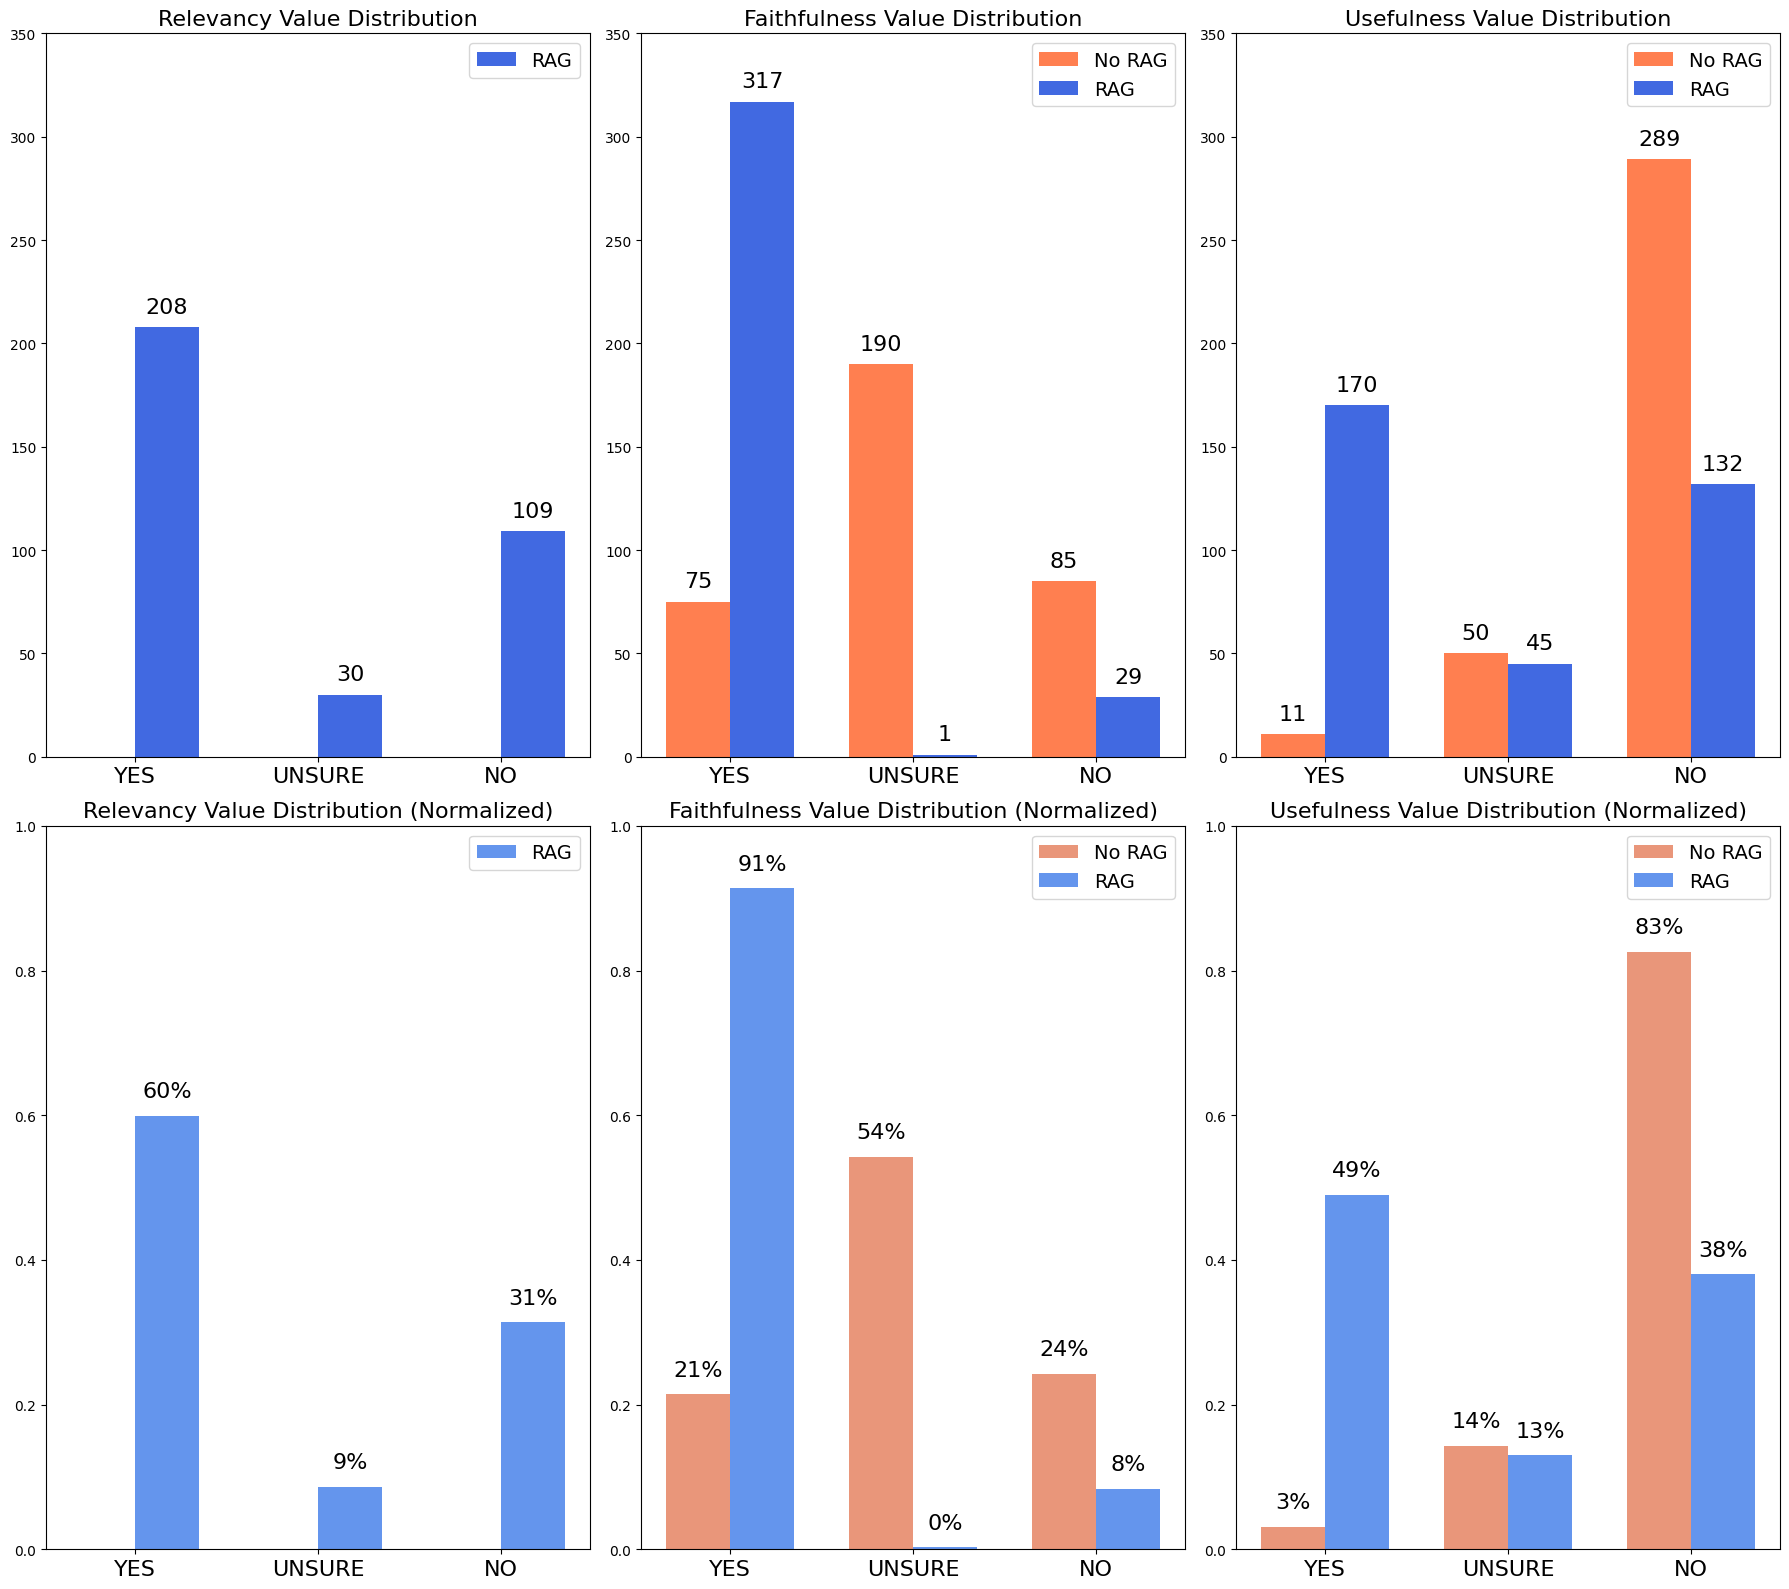
\includegraphics[width=\textwidth,height=\textheight,keepaspectratio]{Figures/RegularQA_res.png}
\caption{The results of the Regular Questions set experiments}
\label{fig:RegularQA_res}
\end{figure}

As can be seen, the use of context (RAG setup) in the system does indeed significantly improve the quality of LLM responses.

We can then analyze in more detail the results of the metrics in terms of each question. The task does not require an absolutely precise approach, but a distribution of averages is sufficient. For this purpose, the assessment results were converted into scores: 0 for “No”, 0.5 for “Unsure”, and 1 for “Yes”. Further, to visualize the results, a heatmap was constructed, which shows the distribution of results by questions. The results are illustrated in the heatmap in the \autoref{fig:results_heatmap}:
\begin{figure}[H]
\centering
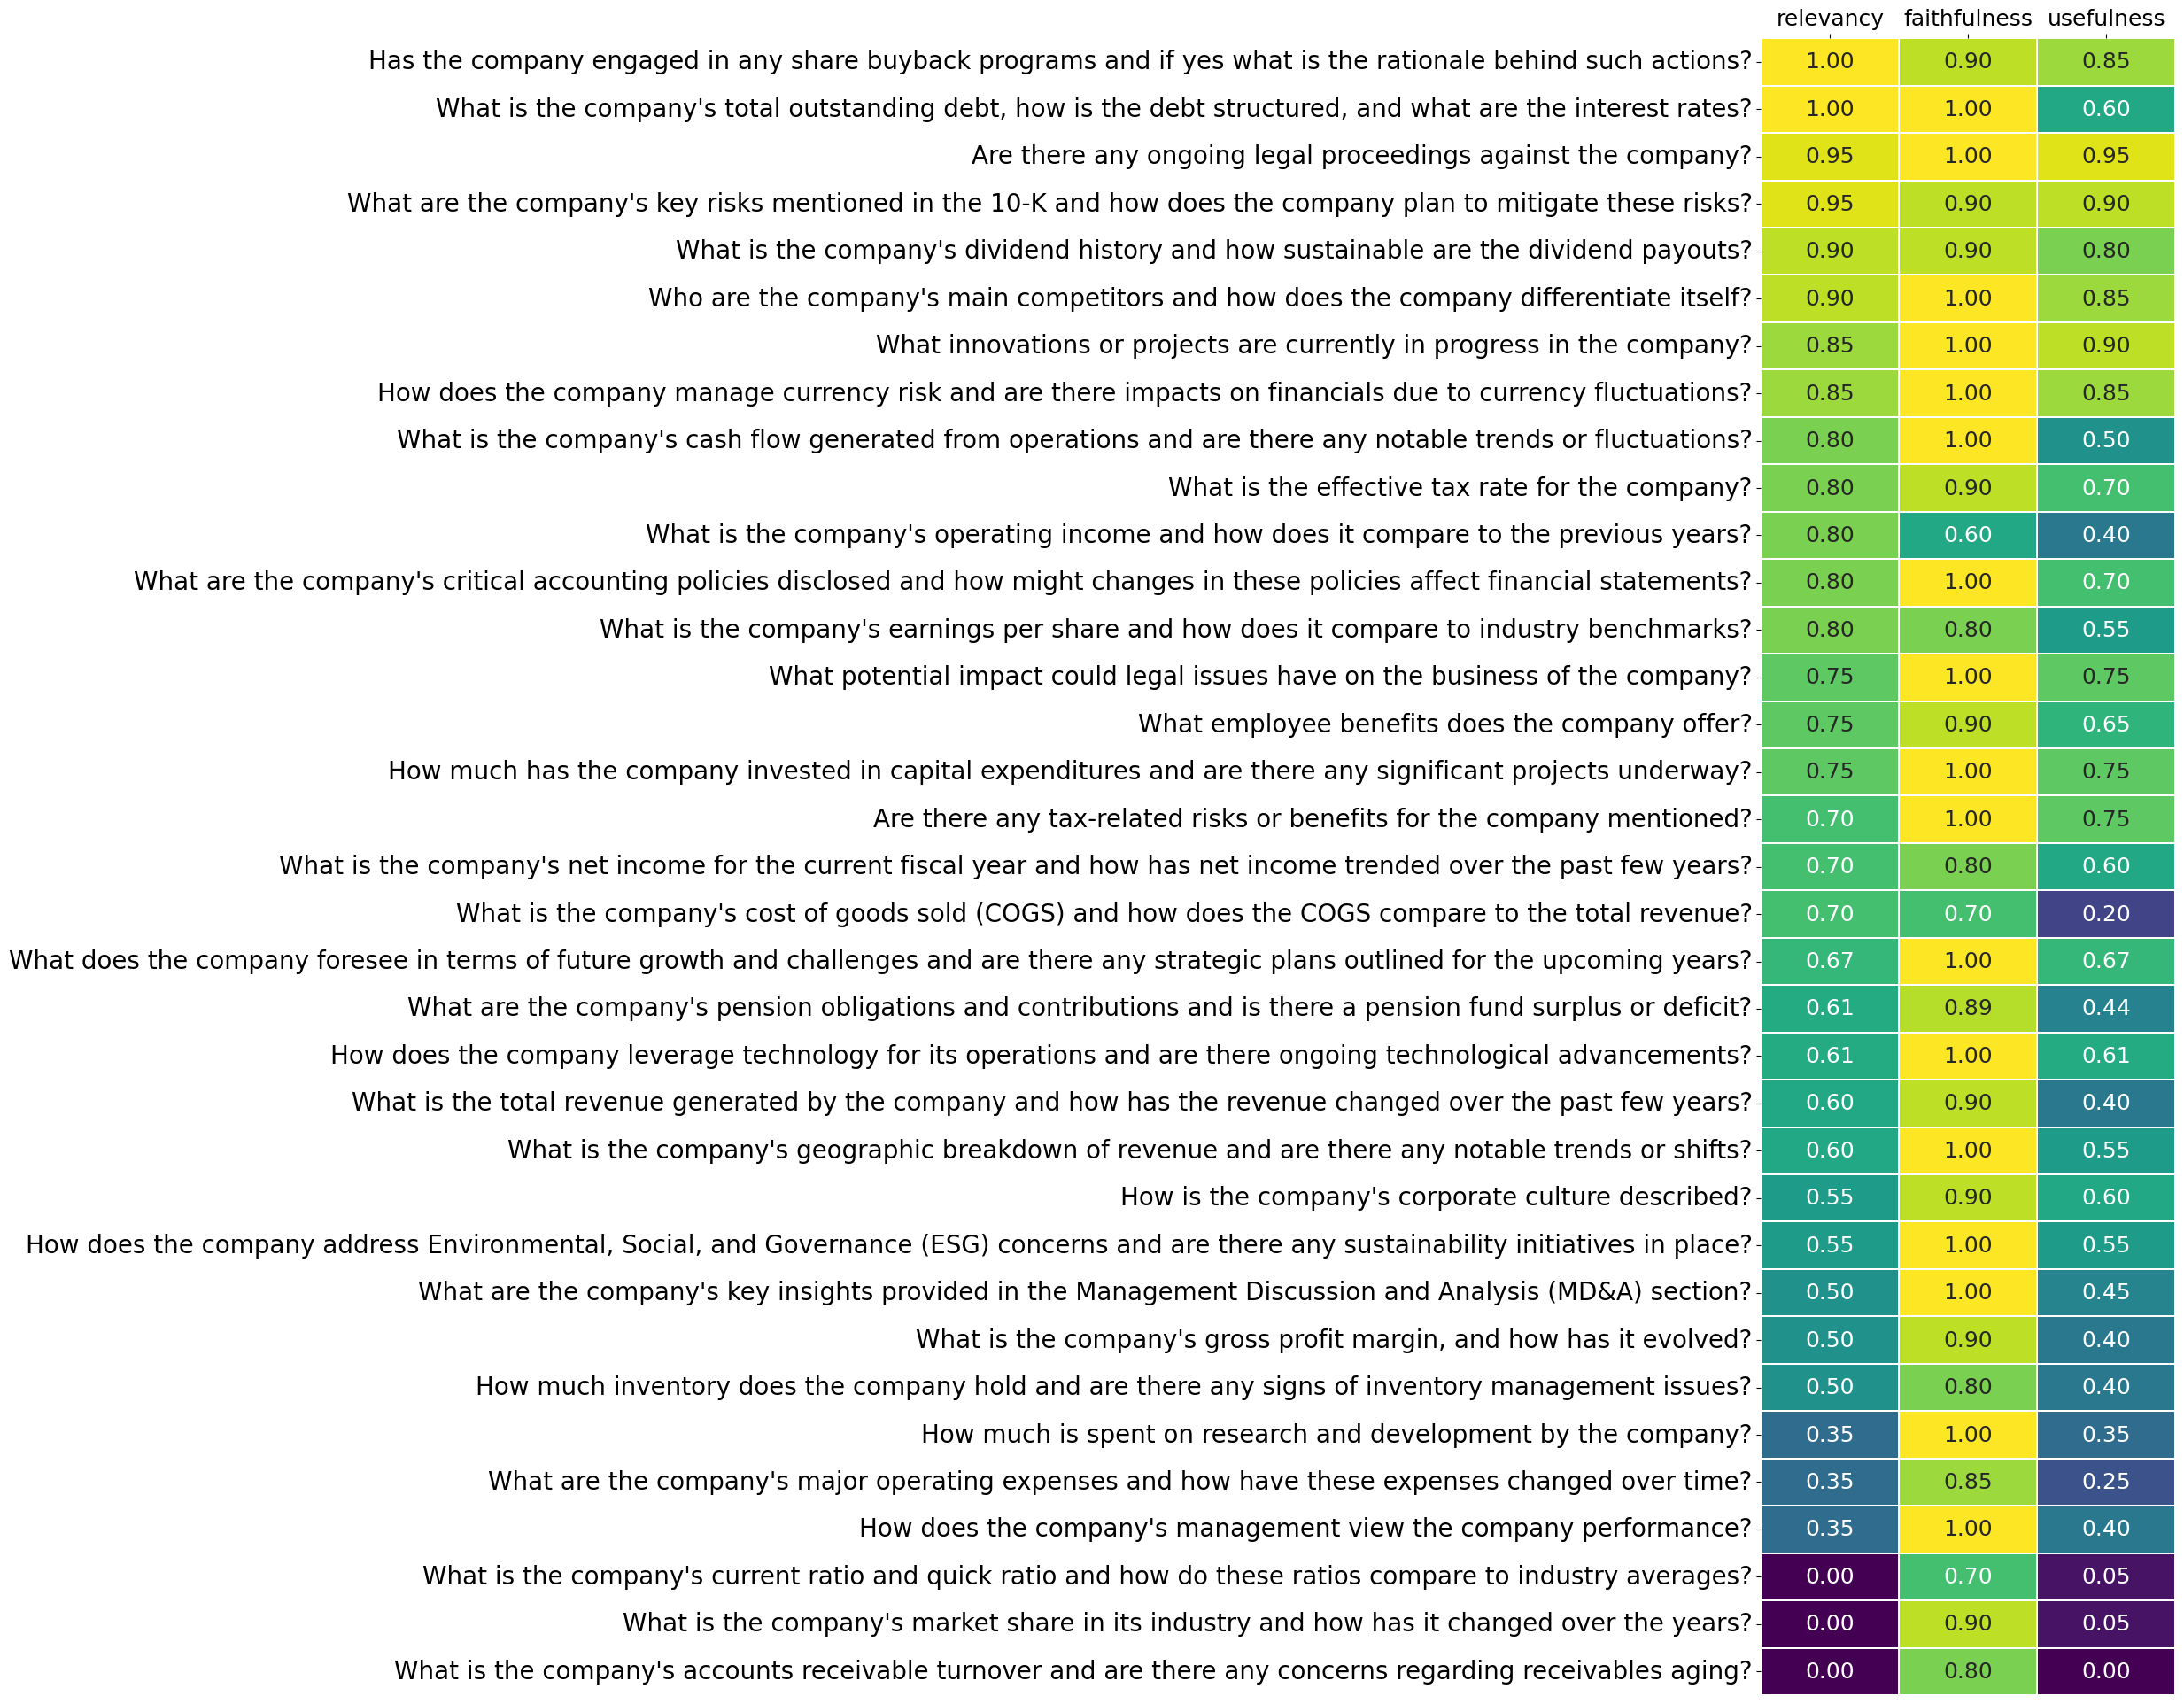
\includegraphics[width=1\textwidth]{Figures/results_heatmap.png}
\caption{The heatmap for the questions accuracy results of the Regular Questions dataset experiments}
\label{fig:results_heatmap}
\end{figure}
\\
The heatmap presents the average relevancy, faithfulness, and usefulness values for each query in the Regular Questions dataset. These metrics provide a quantifiable measure of the quality of the responses generated by the model.

Most queries exhibit high relevancy and faithfulness scores, particularly those related to direct financial information and strategic insights. Queries like "Has the company engaged in any share buyback programs and if yes what is the rationale behind such actions?" and "What is the company's total outstanding debt, how is the debt structured, and what are the interest rates?" scored perfect relevancy and near-perfect faithfulness.

Usefulness scores are more varied compared to relevancy and faithfulness. Some queries with high relevancy and faithfulness still show moderate usefulness, suggesting either that while the responses are accurate and relevant they might lack practical application or depth, or that the responses are not accurate at all. For instance, the query "What is the company's total outstanding debt, how is the debt structured, and what are the interest rates?" has high relevancy and faithfulness but a moderate usefulness score of 0.6.

Certain queries have notably low scores across all metrics. For example, "What is the company's current ratio and quick ratio and how do these ratios compare to industry averages?" shows zero relevancy and usefulness, indicating a significant gap in the model's ability to address this type of question. Queries related to market share and accounts receivable turnover also score very low, suggesting the need for improved data retrieval or response generation strategies for these topics. 

Some queries maintain a balanced performance across all metrics, such as "What are the company's key risks mentioned in the 10-K and how does the company plan to mitigate these risks?", which shows high scores in relevancy (0.95), faithfulness (0.9), and usefulness (0.9).

Main conclusions and insights about the Regular Questions set experiments results:
\begin{enumerate}
\item The RAG pipeline performs well in retrieving and generating relevant, faithful, and useful answers for questions related to financial metrics, corporate structure, and competitive analysis.
\item The pipeline struggles with more subjective or complex queries, such as those related to market share, management perspectives, and future growth predictions.
\item Evaluating outcomes is challenging due to the absence of ground truth values for comparison. Thus, we are essentially measuring precision without the ability to measure recall.
\item Some LLM responses include data from the given context but erroneously apply it to other indicators.
\item Some questions lack the necessary information for an answer. In these cases, the retrieved context is evaluated as irrelevant, leading to no distinction between reports that do not contain the information at all and those where retrieval provided an irrelevant document.
\item The "Key Risks" section in reports is often lengthy, containing several pages describing possible risks. The RAG chain is limited by the number of contexts set by the hyperparameter "NUM\_CHUNKS" (set to 2 in our experiments) and by the LLM context window (4,000 tokens for the Phi-3 model). This limitation affects the quality of the final response, typically resulting in the LLM response covering only part of the necessary information.
\end{enumerate}

\subsubsection{Evaluation and Results for the FinanceBench questions set}
A second evaluation was conducted on the FinanceBench Questions set, which comprises 150 questions. For the FinanceBench Questions set the questions, retrieved context (whether relevant or irrelevant to the question), generated responses and ground truth answers were saved as a CSV file. This dataset was then uploaded to the Argilla workspace (a framework that utilizes HuggingFace space) for manual annotation. The dataset was evaluated using the following metrics, with set of ["YES", "NO", "UNSURE"] possible answers for each question:
\begin{enumerate}
\item Usefulness metric. The answer to the question "Is generated answer useful to resolve a question?". If the answer is incorrect or irrelevant, it is not useful. If the response merely indicates where the requested data can be obtained, it is considered unhelpful. A 'YES' for the 'usefulness' metric indicates correct answers or answers containing some correct information. 'NO' also includes factually incorrect answers and responses where the context does not contain relevant information, and the LLM's answer is simply "I do not know" or "I do not have specific information".
\item Correctness metric. The answer to the question "Does the generated answer match the ground truth answer?". The Financebench dataset provides the correct (ground truth) answers to the question. When answering the question, the correct (ground truth) answer was compared to the answer provided by the system.
\end{enumerate}

After all the results of the experiments with FinanceBench Questions set were evaluated on Argilla workspace, the results were analyzed. The distribution of responses between the metrics is shown in the \autoref{table:comparison_FB}:
\begin{table}[H]
\centering
\begin{tabular}{|c|c|c|c|c|}
\hline
\textbf{Metric} & \textbf{Setup} & \textbf{YES} & \textbf{UNSURE} & \textbf{NO} \\ 
\hline
\multirow{2}{*}{Usefulness} & No RAG & 10 (7\%) & 8 (5\%) & 132 (88\%) \\ \cline{2-5}
 & RAG & 25 (17\%) & 15 (10\%) & 110 (73\%) \\
\hline
\multirow{2}{*}{Correctness} & No RAG & 7 (5\%) & 15 (10\%) & 128 (85\%) \\ \cline{2-5}
 & RAG & 20 (13\%) & 11 (7\%) & 119 (79\%) \\
\hline
\end{tabular}
\caption{Comparison of Usefulness and Correctness between No\_RAG and RAG setups}
\label{table:comparison_FB}
\end{table}
The RAG system improves the correctness (from 5\% with No RAG setup to 13\% with RAG setup) and usefulness (from 7\% without RAG to 17\% with RAG) of the LLM-generated answers.

The distribution of the results are shown in the \autoref{fig:results_financebench150}:
\begin{figure}[H]
\centering
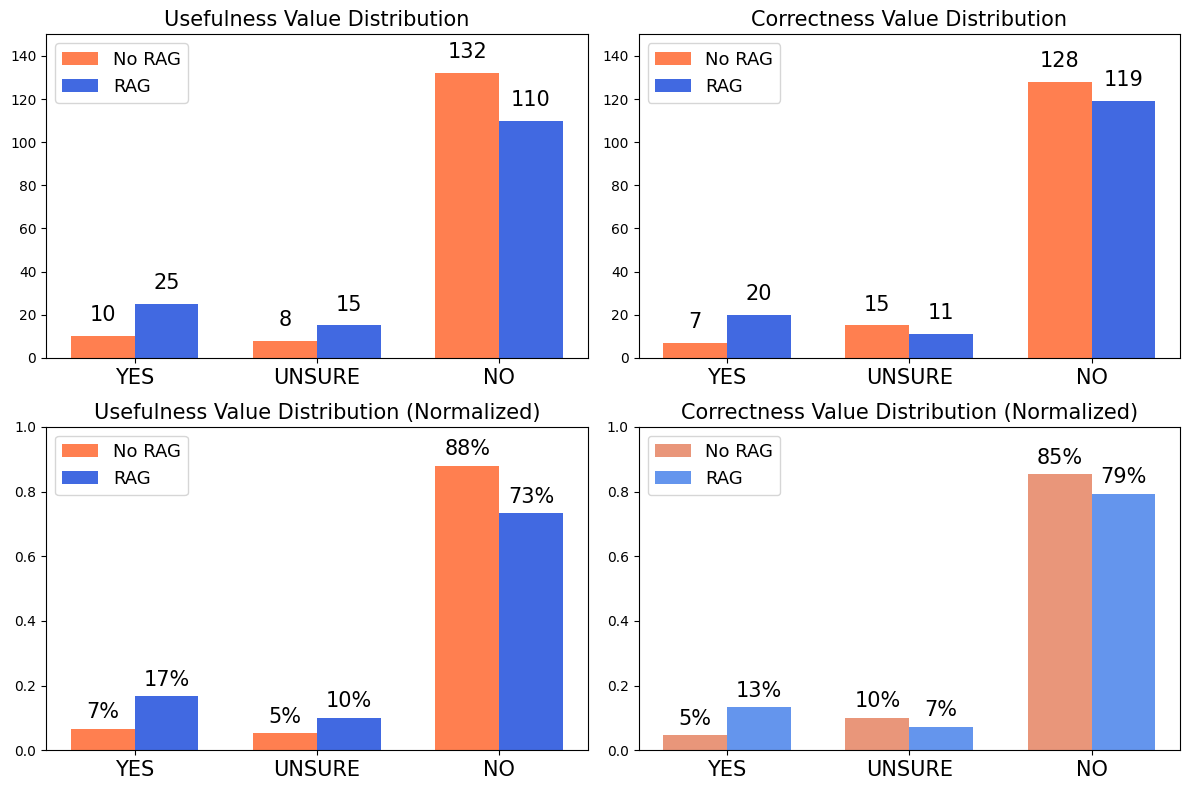
\includegraphics[width=1\textwidth]{Figures/results_financebench150.png}
\caption{The results of the Financebench Questions set experiments}
\label{fig:results_financebench150}
\end{figure}

Without access to additional information (No RAG setup), in a closed book configuration, LLM performs poorly on the Financebench Questions set, phi-3-mini model only gives correct answers to 5\% of questions (the GPT-4-Turbo model in the same closed book configuration gives correct answers to 9\% of prompts \cite{Islam.20Nov2023}), and in a RAG configuration the results are up to 13\%.

The results of the experiments show that 86\% of answers with RAG setup were incorrect (total 'UNSURE' and 'NO' answers), which is very similar to the results obtained by the authors of the Financebench paper with state-of-the-art models. According to the Financebench paper authors tested different LLM configurations including GPT-4-Turbo, Llama2, and Claude2, with and without vector stores and long context prompts, on a FinanceBench questions set and manually reviewed their answers. The best results are from GPT-4-Turbo in oracle setup (with access to evidence pages of the financial reports) with 85\% accuracy. But such a system is impossible in real life. The same GPT-4-Turbo with long context (the whole report was provided to the LLM as context) setup has 79\% accuracy. Single vector store (one vector database for each report) with GPT-4-Turbo has 50\% correct answers, and with Llama 2 - 41\%. And shared vector store systems (one vectorbase for all reports) with both GPT-4-Turbo and Llama 2 models have the same accuracy of 19\%. Existing LLMs have clear limitations for financial questions \cite{Islam.20Nov2023}. 

The RAG pipeline shows the worst results (lowest precision) when answering questions that contain complex queries or multiple sub-questions, especially when the terms are not present in the reports. At the same time if the presented context is of high quality the RAG pipeline is capable of formulating answers to complex queries. In most cases, the reason for an answer being useless is the lack of specific information needed to respond. These indicate that the retrieval stage is crucial for the system's overall performance.

RAG setup helps in answering financial questions, but introduces many related problems, particularly with reasoning. RAG functions well as a search engine, but not as a definitive source of answers. It seems that end-to-end answering of questions is not feasible at this stage. For a RAG system, it is very difficult to capture all important references from a question.

\newpage
\section{Discussions}
The RAG pipeline has significantly improved the performance of the LLM by grounding responses in relevant external context. However, the results are far from perfect and several challenges and unresolved issues remain that need to be addressed for better performance.

The success of RAG heavily depends on the relevance and quality of the retrieved documents. If the retrieval mechanism brings back irrelevant or low-quality documents, the generation process can be adversely affected, leading to inaccurate or irrelevant responses. It is crucial to improve retrieval algorithms to better assess and rank document relevance for enhancing RAG performance.

RAG models sometimes struggle with ambiguous or highly diverse queries that do not have a clear, single relevant document. Enhancing RAG’s ability to handle such queries is necessary for providing more accurate responses. As part of an experiment conducted\footnote{\url{https://github.com/winterForestStump/thesis/blob/main/notebooks/question_rag_x_phi3_experiment.ipynb}}, the question "What is the company's total outstanding debt, how is the debt structured, and what are the interest rates?" was re-asked to the RAG system for about 10 companies (the same companies used in the main experiments), and since the question actually consists of three relatively independent sub-questions "What is the company's total outstanding debt?", "How is the company's debt structured?", "What are the interest rates for company's debt?", each sub-question was also asked to the system. The results obtained were evaluated using the same methodology as the main experiments (described in detail in the Experiments and Results section). The average results obtained for each metric and question are summarized in the heatmap\footnote{\url{https://github.com/winterForestStump/thesis/blob/main/evaluation/question_bge-reranker_x_phi3-4k/question_partition__eval_results.ipynb}} on \autoref{fig:question_partition_heatmap}:
\begin{figure}[h!]
\centering
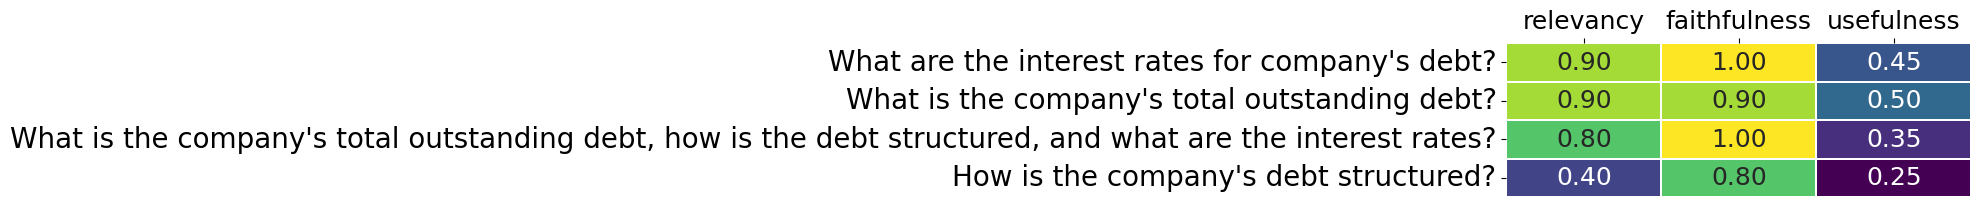
\includegraphics[width=1\textwidth]{Figures/question_partition_heatmap.png}
\caption{The heatmap for the question partition experiment}
\label{fig:question_partition_heatmap}
\end{figure}
The results show that two of the three sub-questions have mean higher than that of the main question. This is especially true for 'relevancy' and 'usefulness'. It can be assumed that the debt structure question is problematic for the system and affects more the decrease of the metrics for the main question. However, this issue requires further investigation.

Retrieval granularity denotes the retrieval unit in which the corpus is indexed, such as documents, passages, or tokens. For RAG, the choice of retrieval granularity can significantly impact performance. Larger chunks capture more context but generate more noise, requiring longer processing time and higher costs. Smaller chunks, while less noisy, may not fully convey the necessary context. Optimizing a recursive splits and sliding window method can help balance semantic completeness and context length. Furthermore, document chunking based on structure instead of paragraphs can improve the quality of RAG's outputs \cite{Yepes.5Feb2024}.

One of the primary limitations of current RAG architectures is their inability to integrate content from previous conversation turns. Each response is generated based solely on the immediate input query, without considering the dialogue history. This limitation can result in a lack of continuity and coherence, as the model cannot reference or build upon previous turns. The model might provide inconsistent responses since it doesn't have the context of earlier interactions to ensure alignment. Effective incorporation of conversation history is essential for more human-like interactions.

The feature encoder always plays a vital role in natural language processing tasks. Better embedding models are more likely to fetch similarities across contexts and help identify highly relevant context \cite{Dong.28May2024}. Various approaches to embeddings can significantly impact the performance of RAG systems. Although we did not conduct experiments with different chunking strategies and embedding models, it is evident that more advanced approaches could yield substantially different results. For instance, an element-based chunking strategy improved performance in state-of-the-art Q\&A tasks on the FinanceBench Questions dataset \cite{Yepes.5Feb2024}. This improvement was achieved by adopting a better chunking strategy for processing documents, compared to baseline chunking strategies using fixed chunk sizes of 128, 256, and 512 tokens. 

In experiments evaluating the quality of context retrieval from databases, non-manual human evaluations were conducted using LLM. However, the quality of such evaluations may not align with human perception. Since the LLM's task was not rigorously defined and focused mainly on keyword orientation, there is a possibility that the evaluation results could be overestimated. Furthermore, the inconsistency observed in LLM performance across various experiments suggests that the quality of these evaluations could be compromised. Current evaluation metrics may not fully capture the improvements or limitations of RAG models. There is a notable lack of research dedicated to evaluating the unique characteristics of RAG models \cite{Gao.18Dec2023}. Developing more comprehensive and fine-grained evaluation methods that consider aspects such as coherence, relevance, factual accuracy, and user satisfaction is crucial for better assessing and guiding the development of RAG systems.

\newpage
\section{Conclusions}
The aim of this thesis was to explore and develop a RAG system to enhance the reading and understanding of financial annual reports using open-source libraries and models. The power of artificial intelligence, especially in finance, has opened up new possibilities for advanced tools like LLMs and RAGs systems to simplify complicated tasks. Corporate annual reports, including SEC Form 10-K filings, provide crucial insights into a company's financial health and operational dynamics but are often lengthy and intricate. This thesis sought to mitigate these challenges by leveraging the capabilities of LLMs combined with information retrieval.

We constructed the RAG pipeline using open-source tools and models, emphasizing the accessibility and cost-effectiveness of this approach. Key components of the pipeline included ChromaDB, LangChain and HuggingFace, which were used to deploy a vector database with embedded vectors of the companies' reports, create a retriever for the most relevant content to user queries, and use LLM to generate responses. Our system was tested locally (running the model with LlamaCpp) on a Google Colab virtual machine, avoiding third-party API calls and ensuring data security.

A significant part of our research involved experimenting with various distance metrics to determine the best fit for database similarity searches. The main experiments with RAG system involved two distinct question datasets: Regular Questions and FinanceBench Questions. The results were manually evaluated based on the quality of retrieval, faithfulness of answers (grounded on the provided context), and their overall usefulness (correctness, completeness, and relevance) for the Regular Questions answers and based on the usefulness and correctness for the FinanceBench answers.

Our findings indicate that the RAG system can provide reasonable and useful answers, adding significant value to the baseline closed-book LLM's answers by incorporating additional knowledge into the responses. However, it is not yet reliable enough to completely replace human involvement in the question-answering process. Human oversight remains crucial to verify the accuracy of the results, particularly given the tendency of LLMs to generate plausible but factually incorrect information.

The RAG system demonstrated notable improvements in the usefulness of the answers compared to settings without RAG, highlighting the critical role of retrieval quality. High-quality context retrieval directly correlates with the quality of the generated responses, underscoring the importance of continued advancements in retrieval techniques and the overall architecture of RAG systems.

This thesis also highlighted the cost considerations associated with LLMs. While utilizing open-source models can mitigate some expenses, the performance gap between these and proprietary models often necessitates additional resources for manual curating the results, fine-tuning the RAG pipeline. Despite these challenges, the adoption of open-source LLMs remains an attractive option due to their flexibility and customization potential.

The thesis refrained from pursuing predictive tasks such as fraud detection or price prediction, focusing instead on the hypothesis that individuals should make these predictions based on reliable information extracted by the RAG system. By doing so, the research aimed to create and evaluate a tool that supports users within the finance reports, including private investors, professional financial experts, and SEC employees, each benefiting from automated and accurate information retrieval.

In conclusion, while the RAG system we developed shows promise in facilitating the understanding of financial annual reports, significant work remains to be done. Enhancements in retrieval methods are paramount, as the quality of retrieved context fundamentally defines the response quality. Future research should focus on improving retrieval techniques, adopting sophisticated RAG architectures, and exploring new methodologies to enhance LLM's responses.

The overarching goal of this project was to demonstrate the viability of a open-source RAG system that could run locally on a user's work computer. This approach democratizes access to advanced artificial intelligence technologies. Our results indicate that while the system adds substantial value, further refinements are necessary to achieve a level of reliability that could reduce human oversight. As the field of artificial intelligence continues to evolve, the integration of LLMs with real-time, verified data sources presents a promising way for making financial information more accessible and actionable. The success of this project lays a foundation for future work aimed at refining and expanding the capabilities of RAG systems in finance and beyond.





\label{EndOfText}

\addcontentsline{toc}{section}{References}
\newpage
%\pagenumbering{Roman}
%\fancyfoot[C]{Page \thepage\ of \pageref{endOfDoc}}
\bibliographystyle{IEEEtran}
\bibliography{IEEEabrv,cites}
\label{endOfDoc}

%\clearpage

%\listoffigures

%\clearpage

%\listoftables

%\clearpage

%\listoflistings

\end{document}